% Options for packages loaded elsewhere
\PassOptionsToPackage{unicode}{hyperref}
\PassOptionsToPackage{hyphens}{url}
\PassOptionsToPackage{dvipsnames,svgnames,x11names}{xcolor}
\documentclass[
  10pt,
  fontset=fandol]{ctexart}
\usepackage{xcolor}
\usepackage[margin=16mm]{geometry}
\usepackage{amsmath,amssymb}
\setcounter{secnumdepth}{-\maxdimen} % remove section numbering
\usepackage{iftex}
\ifPDFTeX
  \usepackage[T1]{fontenc}
  \usepackage[utf8]{inputenc}
  \usepackage{textcomp} % provide euro and other symbols
\else % if luatex or xetex
  \usepackage{unicode-math} % this also loads fontspec
  \defaultfontfeatures{Scale=MatchLowercase}
  \defaultfontfeatures[\rmfamily]{Ligatures=TeX,Scale=1}
\fi
\usepackage{lmodern}
\ifPDFTeX\else
  % xetex/luatex font selection
\fi
% Use upquote if available, for straight quotes in verbatim environments
\IfFileExists{upquote.sty}{\usepackage{upquote}}{}
\IfFileExists{microtype.sty}{% use microtype if available
  \usepackage[]{microtype}
  \UseMicrotypeSet[protrusion]{basicmath} % disable protrusion for tt fonts
}{}
\makeatletter
\@ifundefined{KOMAClassName}{% if non-KOMA class
  \IfFileExists{parskip.sty}{%
    \usepackage{parskip}
  }{% else
    \setlength{\parindent}{0pt}
    \setlength{\parskip}{6pt plus 2pt minus 1pt}}
}{% if KOMA class
  \KOMAoptions{parskip=half}}
\makeatother
\usepackage{longtable,booktabs,array}
\newcounter{none} % for unnumbered tables
\usepackage{calc} % for calculating minipage widths
% Correct order of tables after \paragraph or \subparagraph
\usepackage{etoolbox}
\makeatletter
\patchcmd\longtable{\par}{\if@noskipsec\mbox{}\fi\par}{}{}
\makeatother
% Allow footnotes in longtable head/foot
\IfFileExists{footnotehyper.sty}{\usepackage{footnotehyper}}{\usepackage{footnote}}
\makesavenoteenv{longtable}
\usepackage{graphicx}
\makeatletter
\newsavebox\pandoc@box
\newcommand*\pandocbounded[1]{% scales image to fit in text height/width
  \sbox\pandoc@box{#1}%
  \Gscale@div\@tempa{\textheight}{\dimexpr\ht\pandoc@box+\dp\pandoc@box\relax}%
  \Gscale@div\@tempb{\linewidth}{\wd\pandoc@box}%
  \ifdim\@tempb\p@<\@tempa\p@\let\@tempa\@tempb\fi% select the smaller of both
  \ifdim\@tempa\p@<\p@\scalebox{\@tempa}{\usebox\pandoc@box}%
  \else\usebox{\pandoc@box}%
  \fi%
}
% Set default figure placement to htbp
\def\fps@figure{htbp}
\makeatother
\setlength{\emergencystretch}{3em} % prevent overfull lines
\providecommand{\tightlist}{%
  \setlength{\itemsep}{0pt}\setlength{\parskip}{0pt}}
\usepackage{amsmath,amssymb,mathtools,needspace}
\xeCJKDeclareCharClass{CJK}{"2032,"0400->"04FF,"2160->"216B,"2460->"2473,"25A0,"25C7,"25CB,"25CF}
\IfFontExistsTF{Arial Unicode MS}{\xeCJKsetup{AutoFallBack=true}\setCJKfallbackfamilyfont{\CJKrmdefault}{Arial Unicode MS}}{}
\setcounter{secnumdepth}{0}
\setlength{\emergencystretch}{2em}
\allowdisplaybreaks
\usepackage{bookmark}
\IfFileExists{xurl.sty}{\usepackage{xurl}}{} % add URL line breaks if available
\urlstyle{same}
\hypersetup{
  pdftitle={数值积分与数值微分},
  colorlinks=true,
  linkcolor={Maroon},
  filecolor={Maroon},
  citecolor={Blue},
  urlcolor={Blue},
  pdfcreator={LaTeX via pandoc}}

\title{数值积分与数值微分}
\author{}
\date{}

\begin{document}
\maketitle

\section{第 4 章 数值积分与数值微分}\label{ux7b2c-4-ux7ae0-ux6570ux503cux79efux5206ux4e0eux6570ux503cux5faeux5206}

\subsection{4.1 引言}\label{ux5f15ux8a00}

\subsubsection{4.1.1 数值求积的基本思想}\label{ux6570ux503cux6c42ux79efux7684ux57faux672cux601dux60f3}

有很多实际问题常常需要计算积分才能求解。有些数值方法，如微分方程和积分方程的求解，也都和积分计算有联系。

依据人们所熟知的微积分基本定理，对于积分 \(I=\int_a^b f(x)\,\mathrm{d}x\)，只要找到被积函数 \(f(x)\) 的原函数 \(F(x)\)，便有下列 Newton-Leibniz 公式：

\[
\int_a^b f(x)\,\mathrm{d}x=F(b)-F(a).
\]

但实际使用这种求积方法往往有困难，因为大量的被积函数，诸如 \(\dfrac{\sin x}{x}\)，\(\sin x^2\) 等等，找不到用初等函数表示的原函数；另外，当 \(f(x)\) 是由测量或数值计算给出的一张数据表时，Newton-Leibniz 公式也不能直接运用。因此有必要研究积分的数值计算问题。

积分中值定理告诉我们，在积分区间 \((a,b)\) 内存在一点 \(\xi\)，有下式成立：

\[
\int_a^b f(x)\,\mathrm{d}x=(b-a)f(\xi).
\]

就是说，底为 \(b-a\) 而高为 \(f(\xi)\) 的矩形面积恰等于所求曲边梯形的面积 \(I\)（见图 4.1）。问题在于点 \(\xi\) 的具体位置一般是不知道的，因而难以准确算出 \(f(\xi)\) 的值。我们将 \(f(\xi)\) 称为区间 \([a,b]\) 上的平均高度。这样，只要对平均高度 \(f(\xi)\) 提供一种算法，相应地便获得一种数值求积方法。

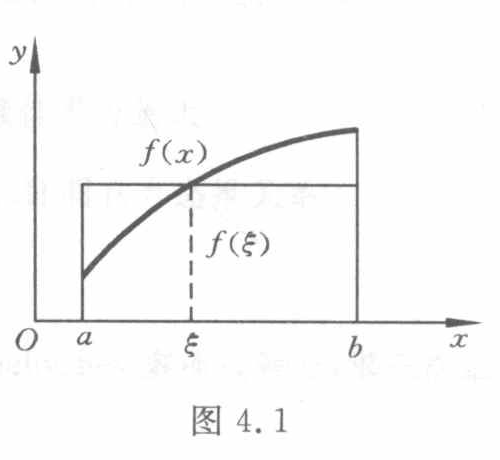
\includegraphics[width=0.85\linewidth,height=\textheight,keepaspectratio,alt={图 4.1（原图裁切）}]{../assets/ch04a/fig-4-1.png}

图 4.1（原图）。图意说明（agent 补充）：曲线 \(f(x)\) 下方从 \(a\) 到 \(b\) 的曲边梯形，与高为 \(f(\xi)\) 的矩形面积相等。图中符号标签：\(x\)，\(y\)，\(O\)，\(a\)，\(\xi\)，\(b\)，\(f(x)\)，\(f(\xi)\)。

如果用两端点的``高度'' \(f(a)\) 与 \(f(b)\) 取算术平均作为平均高度 \(f(\xi)\) 的近似值，这样导出的求积公式

\[
T=\frac{b-a}{2}[f(a)+f(b)]
\tag{4.1.1}
\]

便是我们所熟悉的梯形公式（几何意义参见图 4.2）。如果改用区间中点 \(c=\dfrac{a+b}{2}\) 的

\href{../../source-images/pdf-094.jpeg}{原页图像}

``高度'' \(f(c)\) 近似地取代平均高度 \(f(\xi)\)，则又可导出所谓中矩形公式（以下简称矩形公式）

\[
R=(b-a)f\left(\frac{a+b}{2}\right).
\tag{4.1.2}
\]

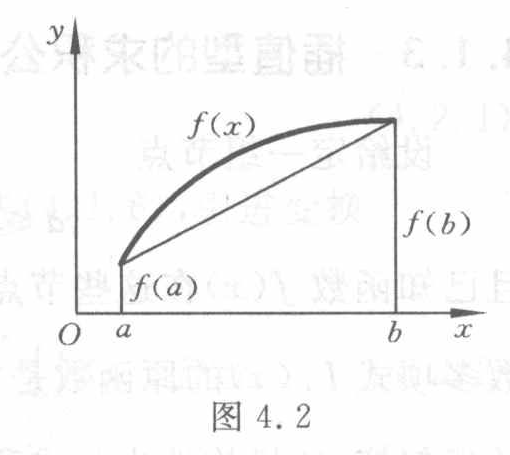
\includegraphics[width=0.85\linewidth,height=\textheight,keepaspectratio,alt={图 4.2（原图裁切）}]{../assets/ch04a/fig-4-2.png}

图 4.2（原图）。图意说明（agent 补充）：用连接曲线 \(f(x)\) 在 \(a\)、\(b\) 两端点的线段形成的梯形近似曲边梯形。图中符号标签：\(x\)，\(y\)，\(O\)，\(a\)，\(b\)，\(f(x)\)，\(f(a)\)，\(f(b)\)。

更一般地，可以在区间 \([a,b]\) 上适当选取某些节点 \(x_k\)，然后用 \(f(x_k)\) 加权平均得到平均高度 \(f(\xi)\) 的近似值，这样构造出的求积公式具有下列形式：

\[
\int_a^b f(x)\,\mathrm{d}x\approx\sum_{k=0}^n A_k f(x_k).
\tag{4.1.3}
\]

其中 \(x_k\) 称为求积节点；\(A_k\) 称为求积系数，亦称伴随节点 \(x_k\) 的权。权 \(A_k\) 仅仅与节点 \(x_k\) 的选取有关，而不依赖于被积函数 \(f(x)\) 的具体形式。

这类数值积分方法通常称为机械求积，其特点是将积分求值问题归结为函数值的计算，这就避开了 Newton-Leibniz 公式需要寻求原函数的困难。

\subsubsection{4.1.2 代数精度的概念}\label{ux4ee3ux6570ux7cbeux5ea6ux7684ux6982ux5ff5}

数值求积方法是近似方法，为保证精度，自然希望求积公式对于``尽可能多''的函数都能准确地成立，这就提出了所谓代数精度的概念。

\textbf{定义 4.1} 如果某个求积公式对于次数不大于 \(m\) 的多项式均能准确地成立，但对于 \(m+1\) 次多项式就不一定准确，则称该求积公式具有 \(m\) 次代数精度。

不难验证，梯形公式（4.1.1）和矩形公式（4.1.2）均具有一次代数精度。

一般地，欲使求积公式（4.1.3）具有 \(m\) 次代数精度，只要令它对于 \(f(x)=1,x,x^2,\cdots,x^m\) 都能准确地成立，这就要求

\[
\begin{cases}
\displaystyle\sum A_k=b-a,\\[4pt]
\displaystyle\sum A_kx_k=\frac12(b^2-a^2),\\
\qquad\vdots\\
\displaystyle\sum A_kx_k^m=\frac{1}{m+1}(b^{m+1}-a^{m+1}).
\end{cases}
\tag{4.1.4}
\]

为简洁起见，这里省略了符号 \(\displaystyle\sum_{k=0}^n\) 中的上、下限。

如果事先选定求积节点 \(x_k\)，譬如，以区间 \([a,b]\) 的等距分点作为节点，这时取 \(m=n\) 求解方程组（4.1.4）即可确定求积系数 \(A_k\)，而使求积公式（4.1.3）至少具有 \(n\) 次代数精度。4.2 节将介绍这样一类求积公式，梯形公式作为其中的一个特例。

构造出形如式（4.1.3）的求积公式的问题，原则上是个确定参数 \(x_k\) 和 \(A_k\) 的代数问题。

\href{../../source-images/pdf-095.jpeg}{原页图像}

\subsubsection{4.1.3 插值型的求积公式}\label{ux63d2ux503cux578bux7684ux6c42ux79efux516cux5f0f}

设给定一组节点

\[
a\leq x_0<x_1<x_2<\cdots<x_n\leq b
\]

且已知函数 \(f(x)\) 在这些节点上的值，作插值函数 \(L_n(x)\)（参见式（2.2.11））。由于代数多项式 \(L_n(x)\) 的原函数是容易求出的，取 \(I_n=\int_a^b L_n(x)\,\mathrm{d}x\) 作为积分 \(I=\int_a^b f(x)\,\mathrm{d}x\) 的近似值，这样构造出的求积公式

\[
I_n=\sum_{k=0}^n A_kf(x_k)
\tag{4.1.5}
\]

是插值型的，其中求积系数 \(A_k\) 通过插值基函数 \(l_k(x)\) 积分

\[
A_k=\int_a^b l_k(x)\,\mathrm{d}x
\tag{4.1.6}
\]

得出。

由插值余项定理（定理 2.2）即知，对于插值型的求积公式（4.1.5），其余项

\[
R[f]=I-I_n=\int_a^b\frac{f^{n+1}(\xi)}{(n+1)!}w(x)\,\mathrm{d}x,
\tag{4.1.7}
\]

其中 \(\xi\) 与变量 \(x\) 有关，\(w(x)=(x-x_0)(x-x_1)\cdots(x-x_n)\)。

如果求积公式（4.1.5）是插值型的，按式（4.1.7），对于次数不大于 \(n\) 的多项式 \(f(x)\)，其余项 \(R[f]\) 等于零，因而这时求积公式至少具有 \(n\) 次代数精度。

反之，如果求积公式（4.1.5）至少具有 \(n\) 次代数精度，则它必定是插值型的。事实上，这时式（4.1.5）对于插值基函数 \(l_k(x)\) 应准确成立，即有

\[
\int_a^b l_k(x)\,\mathrm{d}x=\sum_{j=0}^n A_jl_k(x_j).
\]

注意到 \(l_k(x_j)=\delta_{kj}\)，上式右端实际上即等于 \(A_k\)，因而式（4.1.6）成立。

综上所述，得到如下结论。

\textbf{定理 4.1} 形如式（4.1.5）的求积公式至少有 \(n\) 次代数精度的充分必要条件是，它是插值型的。

\begin{quote}
校注（agent 补充）：式（4.1.7）原扫描将导数阶数印作 \(f^{n+1}(\xi)\)，未带括号；此处按原式保留。由其引用的插值余项定理及上下文，这里表示 \(n+1\) 阶导数。
\end{quote}

\subsection{4.2 Newton-Cotes 公式}\label{newton-cotes-ux516cux5f0f}

\subsubsection{4.2.1 Cotes 系数}\label{cotes-ux7cfbux6570}

设将积分区间 \([a,b]\) 划分为 \(n\) 等份，步长 \(h=\dfrac{b-a}{n}\)，选取等距节点 \(x_k=a+kh\) 构

\href{../../source-images/pdf-096.jpeg}{原页图像}

造出的插值型求积公式

\[
I_n=(b-a)\sum_{k=0}^n C_k^{(n)}f(x_k)
\tag{4.2.1}
\]

称为 Newton-Cotes 公式，其中 \(C_k^{(n)}\) 称为 Cotes 系数。按式（4.1.6），引进变换

\[
x=a+th,
\]

则有

\[
C_k^{(n)}=\frac{h}{b-a}\int_0^n\prod_{\substack{j=0\\j\ne k}}^n\frac{t-j}{k-j}\,\mathrm{d}t
=\frac{(-1)^{n-k}}{nk!(n-k)!}\int_0^n\prod_{\substack{j=0\\j\ne k}}^n(t-j)\,\mathrm{d}t.
\tag{4.2.2}
\]

由于是多项式的积分，Cotes 系数的计算不会遇到实质性的困难。当 \(n=1\) 时，

\[
C_0^{(1)}=C_1^{(1)}=\frac12,
\]

这时求积公式是我们所熟悉的梯形公式（4.1.1）。

当 \(n=2\) 时，按式（4.2.2），Cotes 系数为

\[
C_0^{(2)}=\frac14\int_0^2(t-1)(t-2)\,\mathrm{d}t=\frac16,
\]

\[
C_1^{(2)}=-\frac12\int_0^2t(t-2)\,\mathrm{d}t=\frac46,\qquad
C_2^{(2)}=\frac14\int_0^2t(t-1)\,\mathrm{d}t=\frac16.
\]

相应的求积公式是下列 Simpson 公式：

\[
S=\frac{b-a}{6}\left[f(a)+4f\left(\frac{a+b}{2}\right)+f(b)\right].
\tag{4.2.3}
\]

而 \(n=4\) 的 Newton-Cotes 公式则特别称为 Cotes 公式，其形式为

\[
C=\frac{b-a}{90}[7f(x_0)+32f(x_1)+12f(x_2)+32f(x_3)+7f(x_4)].
\tag{4.2.4}
\]

这里 \(x_k=a+kh\)，\(h=\dfrac{b-a}{4}\)。

表 4.1 列出 Cotes 系数表开头的一部分。

表 4.1

{\def\LTcaptype{none} % do not increment counter
\begin{longtable}[]{@{}
  >{\raggedright\arraybackslash}p{(\linewidth - 12\tabcolsep) * \real{0.1429}}
  >{\raggedright\arraybackslash}p{(\linewidth - 12\tabcolsep) * \real{0.1429}}
  >{\raggedright\arraybackslash}p{(\linewidth - 12\tabcolsep) * \real{0.1429}}
  >{\raggedright\arraybackslash}p{(\linewidth - 12\tabcolsep) * \real{0.1429}}
  >{\raggedright\arraybackslash}p{(\linewidth - 12\tabcolsep) * \real{0.1429}}
  >{\raggedright\arraybackslash}p{(\linewidth - 12\tabcolsep) * \real{0.1429}}
  >{\raggedright\arraybackslash}p{(\linewidth - 12\tabcolsep) * \real{0.1429}}@{}}
\toprule\noalign{}
\begin{minipage}[b]{\linewidth}\raggedright
\(n\)
\end{minipage} & \begin{minipage}[b]{\linewidth}\raggedright
\(C_0^{(n)}\)
\end{minipage} & \begin{minipage}[b]{\linewidth}\raggedright
\(C_1^{(n)}\)
\end{minipage} & \begin{minipage}[b]{\linewidth}\raggedright
\(C_2^{(n)}\)
\end{minipage} & \begin{minipage}[b]{\linewidth}\raggedright
\(C_3^{(n)}\)
\end{minipage} & \begin{minipage}[b]{\linewidth}\raggedright
\(C_4^{(n)}\)
\end{minipage} & \begin{minipage}[b]{\linewidth}\raggedright
\(C_5^{(n)}\)
\end{minipage} \\
\midrule\noalign{}
\endhead
\bottomrule\noalign{}
\endlastfoot
1 & \(\frac12\) & \(\frac12\) & & & & \\
2 & \(\frac16\) & \(\frac23\) & \(\frac16\) & & & \\
3 & \(\frac18\) & \(\frac38\) & \(\frac38\) & \(\frac18\) & & \\
4 & \(\frac7{90}\) & \(\frac{16}{45}\) & \(\frac2{15}\) & \(\frac{16}{45}\) & \(\frac7{90}\) & \\
5 & \(\frac{19}{288}\) & \(\frac{25}{96}\) & \(\frac{25}{144}\) & \(\frac{25}{144}\) & \(\frac{25}{96}\) & \(\frac{19}{288}\) \\
\end{longtable}
}

\href{../../source-images/pdf-097.jpeg}{原页图像}

表 4.1（续表）

{\def\LTcaptype{none} % do not increment counter
\begin{longtable}[]{@{}
  >{\raggedright\arraybackslash}p{(\linewidth - 18\tabcolsep) * \real{0.1000}}
  >{\raggedright\arraybackslash}p{(\linewidth - 18\tabcolsep) * \real{0.1000}}
  >{\raggedright\arraybackslash}p{(\linewidth - 18\tabcolsep) * \real{0.1000}}
  >{\raggedright\arraybackslash}p{(\linewidth - 18\tabcolsep) * \real{0.1000}}
  >{\raggedright\arraybackslash}p{(\linewidth - 18\tabcolsep) * \real{0.1000}}
  >{\raggedright\arraybackslash}p{(\linewidth - 18\tabcolsep) * \real{0.1000}}
  >{\raggedright\arraybackslash}p{(\linewidth - 18\tabcolsep) * \real{0.1000}}
  >{\raggedright\arraybackslash}p{(\linewidth - 18\tabcolsep) * \real{0.1000}}
  >{\raggedright\arraybackslash}p{(\linewidth - 18\tabcolsep) * \real{0.1000}}
  >{\raggedright\arraybackslash}p{(\linewidth - 18\tabcolsep) * \real{0.1000}}@{}}
\toprule\noalign{}
\begin{minipage}[b]{\linewidth}\raggedright
\(n\)
\end{minipage} & \begin{minipage}[b]{\linewidth}\raggedright
\(C_0^{(n)}\)
\end{minipage} & \begin{minipage}[b]{\linewidth}\raggedright
\(C_1^{(n)}\)
\end{minipage} & \begin{minipage}[b]{\linewidth}\raggedright
\(C_2^{(n)}\)
\end{minipage} & \begin{minipage}[b]{\linewidth}\raggedright
\(C_3^{(n)}\)
\end{minipage} & \begin{minipage}[b]{\linewidth}\raggedright
\(C_4^{(n)}\)
\end{minipage} & \begin{minipage}[b]{\linewidth}\raggedright
\(C_5^{(n)}\)
\end{minipage} & \begin{minipage}[b]{\linewidth}\raggedright
\(C_6^{(n)}\)
\end{minipage} & \begin{minipage}[b]{\linewidth}\raggedright
\(C_7^{(n)}\)
\end{minipage} & \begin{minipage}[b]{\linewidth}\raggedright
\(C_8^{(n)}\)
\end{minipage} \\
\midrule\noalign{}
\endhead
\bottomrule\noalign{}
\endlastfoot
6 & \(\frac{41}{840}\) & \(\frac9{35}\) & \(\frac9{280}\) & \(\frac{34}{105}\) & \(\frac9{280}\) & \(\frac9{35}\) & \(\frac{41}{840}\) & & \\
7 & \(\frac{751}{17280}\) & \(\frac{3577}{17280}\) & \(\frac{1323}{17280}\) & \(\frac{2989}{17280}\) & \(\frac{2989}{17280}\) & \(\frac{1323}{17280}\) & \(\frac{3577}{17280}\) & \(\frac{751}{17280}\) & \\
8 & \(\frac{989}{28350}\) & \(\frac{5888}{28350}\) & \(\frac{-928}{28350}\) & \(\frac{10496}{28350}\) & \(\frac{-4540}{28350}\) & \(\frac{10496}{28350}\) & \(\frac{-928}{28350}\) & \(\frac{5888}{28350}\) & \(\frac{989}{28350}\) \\
\end{longtable}
}

可以看到，当 \(n\geq8\) 时，Cotes 系数有正有负，这时稳定性得不到保证。因此，实际计算中不用高阶的 Newton-Cotes 公式。

\begin{quote}
校注（agent 补充，CH04A-E01）：上述``当 \(n\geq8\) 时''若理解为对所有这类整数 \(n\) 成立，则存在原书表述错误。保留原文。由式（4.2.2）直接积分，\(n=9\) 时系数为 \[
\left(\frac{2857}{89600},\frac{15741}{89600},\frac{27}{2240},\frac{1209}{5600},\frac{2889}{44800},\frac{2889}{44800},\frac{1209}{5600},\frac{27}{2240},\frac{15741}{89600},\frac{2857}{89600}\right),
\] 全部为正；\(n=8\) 出现负系数这一事实仍成立。上述反例为 agent 按原公式进行的符号积分核验，不属于原书正文。
\end{quote}

\subsubsection{4.2.2 偶阶求积公式的代数精度}\label{ux5076ux9636ux6c42ux79efux516cux5f0fux7684ux4ee3ux6570ux7cbeux5ea6}

作为插值型的求积公式，\(n\) 阶的 Newton-Cotes 公式至少具有 \(n\) 次的代数精度（见定理 4.1）。实际的代数精度能否进一步提高呢？

先看 Simpson 公式（4.2.3），它是二阶 Newton-Cotes 公式，因此至少具有二次代数精度。进一步用 \(f(x)=x^3\) 进行检验，按 Simpson 公式计算，得

\[
S=\frac{b-a}{6}\left[a^3+4\left(\frac{a+b}{2}\right)^3+b^3\right].
\]

另一方面直接求积得 \(I=\int_a^b x^3\,\mathrm{d}x=\dfrac{b^4-a^4}{4}\)。这时有 \(S=I\)，即 Simpson 公式对次数不超过三次的多项式均能准确成立。又容易验证它对于 \(f(x)=x^4\) 通常是不准确的，因此，Simpson 公式实际上具有三次代数精度。

一般地，可以证明下述论断。

\textbf{定理 4.2} 当阶 \(n\) 为偶数时，Newton-Cotes 公式（4.2.1）至少有 \(n+1\) 次代数精度。

\textbf{证明} 只要验证，当 \(n\) 为偶数时，Newton-Cotes 公式对 \(f(x)=x^{n+1}\) 的余项为零。

按余项公式（4.1.7），由于这里 \(f^{(n+1)}(x)=(n+1)!\)，从而有

\[
R[f]=\int_a^b\prod_{j=0}^n(x-x_j)\,\mathrm{d}x.
\]

引进变换 \(x=a+th\)，并注意到 \(x_j=a+jh\)，有

\[
R[f]=h^{n+2}\int_0^n\prod_{j=0}^n(t-j)\,\mathrm{d}t.
\]

若 \(n\) 为偶数，则 \(\dfrac n2\) 为整数，再令 \(t=u+\dfrac n2\)，进一步有

\[
R[f]=h^{n+2}\int_{-n/2}^{n/2}\prod_{j=0}^n\left(u+\frac n2-j\right)\,\mathrm{d}u,
\]

\href{../../source-images/pdf-098.jpeg}{原页图像}

据此可以断定 \(R[f]=0\)，因为被积函数

\[
H(u)=\prod_{j=0}^n\left(u+\frac n2-j\right)=\prod_{j=-n/2}^{n/2}(u-j)
\]

是个奇函数。证毕。

\subsubsection{4.2.3 几种低阶求积公式的余项}\label{ux51e0ux79cdux4f4eux9636ux6c42ux79efux516cux5f0fux7684ux4f59ux9879}

首先考察梯形公式，按余项公式（4.1.7），梯形公式（4.1.1）的余项为

\[
R_{\mathrm{T}}=I-T=\int_a^b\frac{f''(\xi)}2(x-a)(x-b)\,\mathrm{d}x.
\]

这里积分的核函数 \((x-a)(x-b)\) 在区间 \([a,b]\) 上保号（非正），应用积分中值定理，在 \((a,b)\) 内存在一点 \(\eta\)，使

\[
R_{\mathrm{T}}=\frac{f''(\eta)}2\int_a^b(x-a)(x-b)\,\mathrm{d}x
=-\frac{f''(\eta)}{12}(b-a)^3,\quad\eta\in(a,b).
\tag{4.2.5}
\]

再研究 Simpson 公式（4.2.3）的余项 \(R_{\mathrm{S}}=I-S\)。为此构造次数不大于三的多项式 \(H(x)\)，使之满足

\[
H(a)=f(a),\quad H(b)=f(b),\quad H(c)=f(c),\quad H'(c)=f'(c),
\tag{4.2.6}
\]

这里 \(c=\dfrac{a+b}{2}\)。由于 Simpson 公式具有三次代数精度，它对于这样构造出的三次式 \(H(x)\) 是准确的：

\[
\int_a^b H(x)\,\mathrm{d}x=\frac{b-a}{6}[H(a)+4H(c)+H(b)].
\]

而由插值条件（4.2.6）知，上式右端实际上等于按 Simpson 公式（4.2.3）求得的积分值 \(S\)，因此积分余项

\[
R_{\mathrm{S}}=I-S=\int_a^b[f(x)-H(x)]\,\mathrm{d}x.
\]

不难证明，对于满足条件（4.2.6）的多项式 \(H(x)\)，其插值余项

\[
f(x)-H(x)=\frac{f^{(4)}(\xi)}{4!}(x-a)(x-c)^2(x-b),
\]

故有

\[
R_{\mathrm{S}}=\int_a^b\frac{f^{(4)}(\xi)}{4!}(x-a)(x-c)^2(x-b)\,\mathrm{d}x.
\]

这时积分核 \((x-a)(x-c)^2(x-b)\) 在 \([a,b]\) 上保号（非正），用积分中值定理有

\[
R_{\mathrm{S}}=\frac{f^{(4)}(\eta)}{4!}\int_a^b(x-a)(x-c)^2(x-b)\,\mathrm{d}x
=-\frac{b-a}{180}\left(\frac{b-a}{2}\right)^4f^{(4)}(\eta).
\tag{4.2.7}
\]

关于 Cotes 公式（4.2.4）的积分余项，这里不再具体推导，仅列出结果如下：

\[
R_{\mathrm{C}}=I-C=-\frac{2(b-a)}{945}\left(\frac{b-a}{4}\right)^6f^{(6)}(\eta).
\tag{4.2.8}
\]

\href{../../source-images/pdf-099.jpeg}{原页图像}

\subsubsection{4.2.4 复化求积法及其收敛性}\label{ux590dux5316ux6c42ux79efux6cd5ux53caux5176ux6536ux655bux6027}

前已指出，在使用 Newton-Cotes 公式时，提高阶的途径并不总能取得满意的效果。为了改善求积的精度，通常采用复化求积法。

设将积分区间 \([a,b]\) 划分为 \(n\) 等份，步长 \(h=\dfrac{b-a}{n}\)，分点为 \(x_k=a+kh\)，\(k=0,1,\cdots,n\)。所谓复化求积法，就是先用低阶的 Newton-Cotes 公式求得每个子区间 \([x_k,x_{k+1}]\) 上的积分值 \(I_k\)，然后再求和，用 \(\displaystyle\sum_{k=0}^{n-1}I_k\) 作为所求积分 \(I\) 的近似值。

复化梯形公式的形式是

\[
T_n=\sum_{k=0}^{n-1}\frac h2[f(x_k)+f(x_{k+1})]
=\frac h2\left[f(a)+2\sum_{k=1}^{n-1}f(x_k)+f(b)\right],
\tag{4.2.9}
\]

依式（4.2.5），其积分余项

\[
I-T_n=\sum_{k=0}^{n-1}\left[-\frac{h^3}{12}f''(\eta_k)\right]
=-\frac{b-a}{12}h^2f''(\eta).
\tag{4.2.10}
\]

此外，记子区间 \([x_k,x_{k+1}]\) 的中点为 \(x_{k+\frac12}\)，则复化 Simpson 公式为

\[
\begin{aligned}
S_n&=\sum_{k=0}^{n-1}\frac h6[f(x_k)+4f(x_{k+\frac12})+f(x_{k+1})]\\
&=\frac h6\left[f(a)+4\sum_{k=0}^{n-1}f(x_{k+\frac12})+2\sum_{k=1}^{n-1}f(x_k)+f(b)\right].
\end{aligned}
\tag{4.2.11}
\]

如果将每个子区间 \([x_k,x_{k+1}]\) 划分为 4 等分，内分点依次记作 \(x_{k+\frac14}\)，\(x_{k+\frac12}\)，\(x_{k+\frac34}\)，则复化 Cotes 公式具有形式

\[
\begin{aligned}
C_n=\frac h{90}\biggl[&7f(a)+32\sum_{k=0}^{n-1}f(x_{k+\frac14})+12\sum_{k=0}^{n-1}f(x_{k+\frac12})\\
&+32\sum_{k=0}^{n-1}f(x_{k+\frac34})+14\sum_{k=1}^{n-1}f(x_k)+7f(b)\biggr].
\end{aligned}
\tag{4.2.12}
\]

依据式（4.2.7）与式（4.2.8），容易得到复化 Simpson 公式和复化 Cotes 公式的余项，它们分别是

\[
I-S_n=-\frac{b-a}{180}\left(\frac h2\right)^4f^{(4)}(\eta),\quad\eta\in[a,b],
\tag{4.2.13}
\]

\[
I-C_n=-\frac{2(b-a)}{945}\left(\frac h4\right)^6f^{(6)}(\eta),\quad\eta\in[a,b].
\tag{4.2.14}
\]

其他 Newton-Cotes 公式亦可用类似的手续加以复化。显然，复化的 Newton-Cotes 公式仍然是形如式（4.1.3）的机械求积公式。

\textbf{例 4.1} 对于函数 \(f(x)=\dfrac{\sin x}{x}\)，试利用表 4.2 计算积分 \(I=\displaystyle\int_0^1\frac{\sin x}{x}\,\mathrm{d}x\)。

\textbf{解} 将积分区间 \([0,1]\) 划分为 8 等份，应用复化梯形法求得 \(T_8=0.945\,690\,9\)；而

\href{../../source-images/pdf-100.jpeg}{原页图像}

如果将 \([0,1]\) 划分为 4 等份，应用复化 Simpson 法有 \(S_4=0.946\,083\,2\)。

比较上面两个结果 \(T_8\) 与 \(S_4\)，它们都需要提供 9 个点上的函数值，计算量基本相同\footnote{使用求积公式时，计算的工作量主要耗费在函数求值上。}，然而精度却差别很大，同积分的准确值\footnote{所谓积分的``准确值''，是指每一位数字都是有效数字的积分值。} \(I=0.946\,083\,1\) 比较，复化梯形法的结果 \(T_8=0.945\,690\,9\) 只有两位有效数字，而复化 Simpson 法的结果 \(S_4=0.946\,083\,2\) 却有六位有效数字。

\begin{quote}
校注（agent 补充，CH04A-E02）：原文``只有两位有效数字''已保留。按本书 1.3.3 的式（1.3.2），以本页所列数值比较，\(|I-T_8|=0.0003922<0.0005\)，而大于 \(0.00005\)；因此 \(T_8\) 应具有三位有效数字。此为数值判断疑误，与原文转录状态分开记录。
\end{quote}

容易证明，复化的梯形法、Simpson 法和 Cotes 法当步长 \(h\to0\) 时均收敛到所求的积分值 \(I\)。现在考察当 \(h\) 很小时误差的渐近性态。

表 4.2

{\def\LTcaptype{none} % do not increment counter
\begin{longtable}[]{@{}ll@{}}
\toprule\noalign{}
\(x\) & \(f(x)\) \\
\midrule\noalign{}
\endhead
\bottomrule\noalign{}
\endlastfoot
\(0\) & \(1\) \\
\(1/8\) & \(0.997\,397\,8\) \\
\(1/4\) & \(0.989\,615\,8\) \\
\(3/8\) & \(0.976\,726\,7\) \\
\(1/2\) & \(0.958\,851\,0\) \\
\(5/8\) & \(0.936\,155\,6\) \\
\(3/4\) & \(0.908\,851\,6\) \\
\(7/8\) & \(0.877\,192\,5\) \\
\(1\) & \(0.841\,470\,9\) \\
\end{longtable}
}

先研究梯形法，按余项公式（4.2.10），有

\[
\frac{I-T_n}{h^2}=-\frac1{12}\sum_{k=0}^{n-1}hf''(\eta_k)\to-\frac1{12}\int_a^b f''(x)\,\mathrm{d}x,
\]

从而当 \(h\to0\) 时有下列渐近关系式：

\[
\frac{I-T_n}{h^2}\to-\frac1{12}[f'(b)-f'(a)].
\]

类似地，对于复化的 Simpson 法和 Cotes 法分别有

\[
\frac{I-S_n}{h^4}\to-\frac1{180\times2^4}[f'''(b)-f'''(a)],
\]

\[
\frac{I-C_n}{h^6}\to-\frac2{945\times4^6}[f^{(5)}(b)-f^{(5)}(a)].
\]

\textbf{定义 4.2} 如果一种复化求积公式 \(I_n\) 当 \(h\to0\) 时成立渐近关系式

\[
\frac{I-I_n}{h^p}\to C\quad(C\ne0,\text{定数}),
\]

则称求积公式 \(I_n\) 是 \(p\) 阶收敛的。

在这种意义下，复化的梯形法、Simpson 法和 Cotes 法分别具有二阶、四阶和六阶收敛精度。而当 \(h\) 很小时，对于复化的梯形法、Simpson 法和 Cotes 法分别有下列误差估计式：

\[
I-T_n\approx-\frac{h^2}{12}[f'(b)-f'(a)],
\tag{4.2.15}
\]

\[
I-S_n\approx-\frac1{180}\left(\frac h2\right)^4[f'''(b)-f'''(a)],
\tag{4.2.16}
\]

\[
I-C_n\approx-\frac2{945}\left(\frac h4\right)^6[f^{(5)}(b)-f^{(5)}(a)].
\tag{4.2.17}
\]

由此可见，若将步长 \(h\) 减半（即等份数 \(n\) 加倍），则梯形法、Simpson 法与 Cotes 法的误差分别减至原有误差的 \(1/4\)、\(1/16\) 与 \(1/64\)。

\href{../../source-images/pdf-101.jpeg}{原页图像}

\subsection{4.3 Romberg 算法}\label{romberg-ux7b97ux6cd5}

\subsubsection{4.3.1 梯形法的递推化}\label{ux68afux5f62ux6cd5ux7684ux9012ux63a8ux5316}

上一节介绍的复化求积方法对提高精度是行之有效的，但在使用求积公式之前必须给出合适的步长。步长太大，精度难以保证；步长太小，又会导致计算量的增加。而事先给出一个恰当的步长往往是困难的。

实际计算中常常采用变步长的计算方案，即在步长逐次分半（即步长二分）的过程中，反复利用复化求积公式进行计算，直至所求得的积分值满足精度要求为止。

下面，我们在变步长的过程中探讨梯形法的计算规律。

设将求积区间 \([a,b]\) 分成 \(n\) 等份，则一共有 \(n+1\) 个分点，按梯形公式（4.2.9）计算积分值 \(T_n\)，需要提供 \(n+1\) 个函数值。如果将求积区间再二分一次，则分点增至 \(2n+1\) 个。将二分前后两个积分值联系起来加以考察，注意到每个子区间 \([x_k,x_{k+1}]\) 经过二分只增加了一个分点 \(x_{k+\frac12}=\dfrac12(x_k+x_{k+1})\)，用复化梯形公式求得该子区间上的积分值为

\[
\frac h4[f(x_k)+2f(x_{k+\frac12})+f(x_{k+1})].
\]

注意，这里 \(h=\dfrac{b-a}{n}\) 代表二分前的步长。将每个子区间上的积分值相加，得

\[
T_{2n}=\frac h4\sum_{k=0}^{n-1}[f(x_k)+f(x_{k+1})]+\frac h2\sum_{k=0}^{n-1}f(x_{k+\frac12}),
\]

从而利用式（4.2.9）可导出下列递推公式：

\[
T_{2n}=\frac12T_n+\frac h2\sum_{k=0}^{n-1}f(x_{k+\frac12}).
\tag{4.3.1}
\]

\textbf{例 4.2} 计算积分值 \(I=\displaystyle\int_0^1\frac{\sin x}{x}\,\mathrm{d}x\)。

\textbf{解} 先对整个区间 \([0,1]\) 使用梯形公式。对于函数 \(f(x)=\dfrac{\sin x}{x}\)，它在 \(x=0\) 的值定义为 \(f(0)=1\)，而 \(f(1)=0.841\,470\,9\)，据梯形公式计算得

\[
T_1=\frac12[f(0)+f(1)]=0.920\,735\,5.
\]

然后将区间二等分，再求出中点的函数值 \(f(1/2)=0.958\,851\,0\)，从而利用递推公式（4.3.1），有

\href{../../source-images/pdf-102.jpeg}{原页图像}

\[
T_2=\frac12T_1+\frac12f\left(\frac12\right)=0.939\,793\,3.
\]

进一步二分求积区间，并计算新分点上的函数值，得

\[
f(1/4)=0.989\,615\,8,\quad f(3/4)=0.908\,851\,6.
\]

再利用式（4.3.1），有

\[
T_4=\frac12T_2+\frac14\left[f\left(\frac14\right)+f\left(\frac34\right)\right]=0.944\,513\,5.
\]

这样不断二分下去，计算结果如表 4.3 所示（表中 \(k\) 代表二分次数，区间等份数 \(n=2^k\)）。

表 4.3

{\def\LTcaptype{none} % do not increment counter
\begin{longtable}[]{@{}
  >{\raggedright\arraybackslash}p{(\linewidth - 10\tabcolsep) * \real{0.1667}}
  >{\raggedright\arraybackslash}p{(\linewidth - 10\tabcolsep) * \real{0.1667}}
  >{\raggedright\arraybackslash}p{(\linewidth - 10\tabcolsep) * \real{0.1667}}
  >{\raggedright\arraybackslash}p{(\linewidth - 10\tabcolsep) * \real{0.1667}}
  >{\raggedright\arraybackslash}p{(\linewidth - 10\tabcolsep) * \real{0.1667}}
  >{\raggedright\arraybackslash}p{(\linewidth - 10\tabcolsep) * \real{0.1667}}@{}}
\toprule\noalign{}
\begin{minipage}[b]{\linewidth}\raggedright
\(k\)
\end{minipage} & \begin{minipage}[b]{\linewidth}\raggedright
1
\end{minipage} & \begin{minipage}[b]{\linewidth}\raggedright
2
\end{minipage} & \begin{minipage}[b]{\linewidth}\raggedright
3
\end{minipage} & \begin{minipage}[b]{\linewidth}\raggedright
4
\end{minipage} & \begin{minipage}[b]{\linewidth}\raggedright
5
\end{minipage} \\
\midrule\noalign{}
\endhead
\bottomrule\noalign{}
\endlastfoot
\(T_n\) & \(0.939\,793\,3\) & \(0.944\,513\,5\) & \(9.945\,690\,9\) & \(0.945\,985\,0\) & \(0.946\,059\,6\) \\
\end{longtable}
}

{\def\LTcaptype{none} % do not increment counter
\begin{longtable}[]{@{}
  >{\raggedright\arraybackslash}p{(\linewidth - 10\tabcolsep) * \real{0.1667}}
  >{\raggedright\arraybackslash}p{(\linewidth - 10\tabcolsep) * \real{0.1667}}
  >{\raggedright\arraybackslash}p{(\linewidth - 10\tabcolsep) * \real{0.1667}}
  >{\raggedright\arraybackslash}p{(\linewidth - 10\tabcolsep) * \real{0.1667}}
  >{\raggedright\arraybackslash}p{(\linewidth - 10\tabcolsep) * \real{0.1667}}
  >{\raggedright\arraybackslash}p{(\linewidth - 10\tabcolsep) * \real{0.1667}}@{}}
\toprule\noalign{}
\begin{minipage}[b]{\linewidth}\raggedright
\(k\)
\end{minipage} & \begin{minipage}[b]{\linewidth}\raggedright
6
\end{minipage} & \begin{minipage}[b]{\linewidth}\raggedright
7
\end{minipage} & \begin{minipage}[b]{\linewidth}\raggedright
8
\end{minipage} & \begin{minipage}[b]{\linewidth}\raggedright
9
\end{minipage} & \begin{minipage}[b]{\linewidth}\raggedright
10
\end{minipage} \\
\midrule\noalign{}
\endhead
\bottomrule\noalign{}
\endlastfoot
\(T_n\) & \(0.946\,076\,9\) & \(0.946\,081\,5\) & \(0.946\,082\,7\) & \(0.946\,083\,0\) & \(0.946\,083\,1\) \\
\end{longtable}
}

积分 \(I\) 的准确值为 \(0.946\,083\,1\)，用变步长方法二分 9 次得到了这个结果。

\begin{quote}
校注（agent 补充，CH04A-E03）：表 4.3 的 \(k=3\) 单元格原扫描确实印为 \(9.945\,690\,9\)，这里按原表保留。由例 4.1 的 \(T_8\) 和本页下段的 \(T_8\) 可知首位应为 \(0\)，即 \(0.945\,690\,9\)，这是原书排印错误。

校注（agent 补充，CH04A-E04）：本页说明 \(k\) 为二分次数，表中 \(k=9\) 为 \(0.946\,083\,0\)，\(k=10\) 才列出 \(0.946\,083\,1\)。故表后``二分 9 次得到了这个结果''与本页表格、次数定义不一致；原句已保留。

校注（agent 补充，CH04A-E07）：表 4.3 的 \(k=5\) 单元格原扫描印为 \(0.946\,059\,6\)，这里按原表保留。对本例 \(f(x)=\sin x/x\)（\(f(0)=1\)）在 \([0,1]\) 上取 \(n=32\) 独立高精度计算复化梯形值，得 \(T_{32}=0.946\,058\,560\,962\,768\,067\ldots\)，保留七位小数应为 \(0.946\,058\,6\)；原表数值有误。
\end{quote}

\subsubsection{4.3.2 Romberg 公式}\label{romberg-ux516cux5f0f}

梯形法的算法简单，但精度较差，收敛的速度缓慢。如何提高收敛速度以节省计算量，自然是人们极为关心的课题。

根据梯形法的误差公式（4.2.15），积分值 \(T_n\) 的截断误差大致与 \(h^2\) 成正比，因此当步长二分后，截断误差将减至原有误差的 \(1/4\)，即有

\[
\frac{I-T_{2n}}{I-T_n}\approx\frac14.
\]

将上式移项整理，可得

\[
I-T_{2n}\approx\frac13(T_{2n}-T_n).
\tag{4.3.2}
\]

由此可见，只要二分前后的两个积分值 \(T_n\) 与 \(T_{2n}\) 相当接近，就可以保证计算结果 \(T_{2n}\) 的误差很小。这种直接用计算结果来估计误差的方法通常称为误差的事后估计法。

按式（4.3.2），积分近似值 \(T_{2n}\) 的误差大致等于 \(\dfrac13(T_{2n}-T_n)\)，因此，如果用这个误差值作为 \(T_{2n}\) 的一种补偿，可以期望，所得到的

\[
\overline T=T_{2n}+\frac13(T_{2n}-T_n)=\frac43T_{2n}-\frac13T_n
\tag{4.3.3}
\]

可能是更好的结果。

再考察例 4.2，所求得的两个梯形值 \(T_4=0.944\,513\,5\) 和 \(T_8=0.945\,690\,9\) 的精

\href{../../source-images/pdf-103.jpeg}{原页图像}

度都很差（与准确值 \(I=0.946\,083\,1\) 比较，只有两三位有效数字），但如果将它们按式（4.3.3）作线性组合，则新的近似值

\[
\overline T=\frac43T_8-\frac13T_4=0.946\,083\,3
\]

却有六位有效数字。

按公式（4.3.3）组合得到的近似值 \(\overline T\)，其实质究竟是什么呢？直接验证易知

\[
S_n=\frac43T_{2n}-\frac13T_n,
\tag{4.3.4}
\]

这就是说，用梯形法二分前后的两个积分值 \(T_n\) 与 \(T_{2n}\)，按式（4.3.3）作线性组合，结果得到 Simpson 法的积分值 \(S_n\)。

再考察 Simpson 法，按误差公式（4.2.16），其截断误差大致与 \(h^4\) 成正比，因此，若将步长折半，则误差将减至原有误差的 \(1/16\)，即有

\[
\frac{I-S_{2n}}{I-S_n}\approx\frac1{16},\quad I\approx\frac{16}{15}S_{2n}-\frac1{15}S_n.
\]

不难直接验证，上式右端的值其实等于 \(C_n\)，就是说，用 Simpson 法二分前后的两个积分值 \(S_n\) 与 \(S_{2n}\)，按式（4.3.3）作线性组合，结果得到 Cotes 法的积分值 \(C_n\)，即

\[
C_n=\frac{16}{15}S_{2n}-\frac1{15}S_n.
\tag{4.3.5}
\]

重复同样的手续，依据 Cotes 法的误差公式（4.2.17）可进一步导出下列 Romberg 公式：

\[
R_n=\frac{64}{63}C_{2n}-\frac1{63}C_n.
\tag{4.3.6}
\]

在变步长的过程中运用式（4.3.4）、式（4.3.5）和式（4.3.6），就能将粗糙的梯形值 \(T_n\) 逐步加工成精度较高的 Simpson 值 \(S_n\)、Cotes 值 \(C_n\) 和 Romberg 值 \(R_n\)。

\textbf{例 4.3} 用加速公式（4.3.4）、（4.3.5）和（4.3.6）加工例 4.2 得到的梯形值，计算结果如表 4.4（\(k\) 代表二分次数）所示。

表 4.4

{\def\LTcaptype{none} % do not increment counter
\begin{longtable}[]{@{}
  >{\raggedright\arraybackslash}p{(\linewidth - 8\tabcolsep) * \real{0.2000}}
  >{\raggedright\arraybackslash}p{(\linewidth - 8\tabcolsep) * \real{0.2000}}
  >{\raggedright\arraybackslash}p{(\linewidth - 8\tabcolsep) * \real{0.2000}}
  >{\raggedright\arraybackslash}p{(\linewidth - 8\tabcolsep) * \real{0.2000}}
  >{\raggedright\arraybackslash}p{(\linewidth - 8\tabcolsep) * \real{0.2000}}@{}}
\toprule\noalign{}
\begin{minipage}[b]{\linewidth}\raggedright
\(k\)
\end{minipage} & \begin{minipage}[b]{\linewidth}\raggedright
\(T_2^k\)
\end{minipage} & \begin{minipage}[b]{\linewidth}\raggedright
\(S_2^{k-1}\)
\end{minipage} & \begin{minipage}[b]{\linewidth}\raggedright
\(C_2^{k-2}\)
\end{minipage} & \begin{minipage}[b]{\linewidth}\raggedright
\(R_2^{k-3}\)
\end{minipage} \\
\midrule\noalign{}
\endhead
\bottomrule\noalign{}
\endlastfoot
0 & \(0.920\,735\,5\) & & & \\
1 & \(0.939\,793\,3\) & \(0.946\,145\,9\) & & \\
2 & \(0.944\,513\,5\) & \(0.946\,086\,9\) & \(0.946\,083\,0\) & \\
3 & \(0.945\,690\,9\) & \(0.946\,083\,3\) & \(0.946\,083\,1\) & \(0.946\,083\,1\) \\
\end{longtable}
}

我们看到，这里利用二分 3 次的数据（它们的精度都很差，只有两三位是有效数字），通过三次加速求得 \(R_1=0.946\,083\,1\)，这个结果的每一位数字都是有效数字，可见加速效果是十分显著的。

\begin{quote}
校注（agent 补充）：表 4.4 的上、下标按原扫描字位保留为 \(T_2^k\)、\(S_2^{k-1}\)、\(C_2^{k-2}\)、\(R_2^{k-3}\)。由本页``\(k\) 代表二分次数''及公式（4.3.4）至（4.3.6），各列数据对应的分段数实际上为 \(2^k\)、\(2^{k-1}\)、\(2^{k-2}\)、\(2^{k-3}\)，即通常记作 \(T_{2^k}\)、\(S_{2^{k-1}}\)、\(C_{2^{k-2}}\)、\(R_{2^{k-3}}\)。另本页由 Simpson 值组合为 Cotes 值的文字仍引用``式（4.3.3）''，已按原文保留；该处实际所列权为 \(16/15\) 和 \(-1/15\)，见式（4.3.5）。
\end{quote}

\href{../../source-images/pdf-104.jpeg}{原页图像}

\subsubsection{4.3.3 Richardson 外推加速法}\label{richardson-ux5916ux63a8ux52a0ux901fux6cd5}

上述加速过程还可以再继续下去，其理论依据是梯形法的余项可展开成下列级数形式。

\textbf{定理 4.3} 设 \(f(x)\in C^\infty[a,b]\)，则成立

\[
T(h)=I+a_1h^2+a_2h^4+a_3h^6+\cdots+a_kh^{2k}+\cdots,
\tag{4.3.7}
\]

其中系数 \(a_k\)（\(k=1,2,\cdots\)）与 \(h\) 无关。

这一余项公式的推导将在 4.3.4 节给出。

按式（4.3.7），有

\[
T\left(\frac h2\right)=I+\frac{\alpha_1}{4}h^2+\frac{\alpha_2}{16}h^4+\frac{\hat\alpha_3}{64}h^6+\cdots.
\tag{4.3.8}
\]

注意，这里的 \(\hat\alpha_k\) 与将要出现的 \(\beta_k\)，\(\gamma_k\) 等均为与 \(h\) 无关的系数。

设将式（4.3.7）与式（4.3.8）按以下方式作线性组合：

\[
T_1(h)=\frac43T\left(\frac h2\right)-\frac13T(h),
\tag{4.3.9}
\]

则可以从余项展开式中消去误差的主要部分 \(h^2\) 项，从而得到

\[
T_1(h)=I+\beta_1h^4+\beta_2h^6+\beta_3h^8+\cdots.
\tag{4.3.10}
\]

比较式（4.3.9）与式（4.3.4）知，这样构造出的 \(\{T_1(h)\}\) 其实就是 Simpson 值序列。

又根据式（4.3.10），有

\[
T_1\left(\frac h2\right)=I+\frac{\beta_1}{16}h^4+\hat\beta_2h^6+\beta_3h^8+\cdots,
\]

若令

\[
T_2(h)=\frac{16}{15}T_1\left(\frac h2\right)-\frac1{15}T_1(h),
\]

则又可进一步从余项展开式中消去 \(h^4\) 项，从而有

\[
T_2(h)=I+\gamma_1h^6+\gamma_2h^8+\cdots.
\]

这样构造出的 \(\{T_2(h)\}\) 其实就是 Cotes 值序列。

如此继续下去，每加速一次，误差的量级便提高二阶。一般地，将 \(T_0(h)=T(h)\) 按公式

\[
T_m(h)=\frac{4^m}{4^m-1}T_{m-1}\left(\frac h2\right)-\frac1{4^m-1}T_{m-1}(h)
\tag{4.3.11}
\]

经过 \(m\)（\(m=1,2,\cdots\)）次加速后，余项便取下列形式：

\[
T_m(h)=I+\delta_1h^{2(m+1)}+\delta_2h^{2(m+2)}+\cdots.
\tag{4.3.12}
\]

上述处理方法通常称为 Richardson 外推加速方法。

设以 \(T_0^{(k)}\) 表示二分 \(k\) 次后求得的梯形值，且以 \(T_m^{(k)}\) 表示序列 \(\{T_0^{(k)}\}\) 的 \(m\) 次加速值，则依递推公式（4.3.11），即

\[
T_m^{(k)}=\frac{4^m}{4^m-1}T_{m-1}^{(k+1)}-\frac1{4^m-1}T_{m-1}^{(k)}\quad(k=1,2,\cdots)
\tag{4.3.13}
\]

\begin{quote}
校注（agent 补充）：式（4.3.8）的系数按原扫描保留为 \(\alpha_1\)、\(\alpha_2\)、\(\hat\alpha_3\)，相邻正文为 \(\hat\alpha_k\)；\(T_1(h/2)\) 的展开式按原扫描保留 \(\hat\beta_2\) 与未带帽的 \(\beta_3\)。这些字形已放大核对，未用常见写法替换原符号。

校注（agent 补充，CH04A-E05）：式（4.3.13）原列 \(k=1,2,\cdots\)，已照录；但下一页的三角表及算法需要计算 \(T_m^{(0)}\)，因而实现同一递推式时也须允许 \(k=0\)。这是原书递推指标范围的缺漏。

校注（agent 补充，CH04A-E06）：仅有 \(f\in C^\infty[a,b]\) 并不能保证式（4.3.7）的无穷级数收敛且等于 \(T(h)\)。在外推分析中应将其理解为 \(h\to0\) 时的渐近展开，即对所需有限阶截断并保留余项；本转录保留原书等式和条件。下一页式（4.3.14）的无穷 Taylor 等式也有同样的光滑性与收敛性区别。
\end{quote}

\href{../../source-images/pdf-105.jpeg}{原页图像}

可以逐行构造出下列三角形数表------\(T\) 数表：

\[
\begin{array}{ccccc}
T_0^{(0)}&&&&\\
T_0^{(1)}&T_1^{(0)}&&&\\
T_0^{(2)}&T_1^{(1)}&T_2^{(0)}&&\\
T_0^{(3)}&T_1^{(2)}&T_2^{(1)}&T_3^{(0)}&\\
\vdots&\vdots&\vdots&\vdots&\ddots
\end{array}
\]

可以证明，如果 \(f(x)\) 充分光滑，那么 \(T\) 数表每一列的元素及对角线元素均收敛到所求的积分值 \(I\)，即

\[
\lim_{k\to\infty}T_m^{(k)}=I\quad(m\text{ 固定}),\quad\lim_{m\to\infty}T_m^{(0)}=I.
\]

电子计算机上的所谓 Romberg 算法，就是在二分过程中逐步形成 \(T\) 数表的具体方法，其步骤如下：

\textbf{步 1} 准备初值。计算 \(T_0^{(0)}=\dfrac{b-a}{2}[f(a)+f(b)]\) 且令 \(1\to k\)（\(k\) 记录二分的次数）。

\textbf{步 2} 求梯形值。按递推公式（4.3.1）计算梯形值 \(T_0^{(k)}\)。

\textbf{步 3} 求加速值。按加速公式（4.3.13）逐个求出 \(T\) 数表第 \(k+1\) 行其余各元素 \(T_j^{(k-j)}\)（\(j=1,2,\cdots,k\)）。

\textbf{步 4} 精度控制。对于指定精度 \(\varepsilon\)，若 \(|T_k^{(0)}-T_{k-1}^{(0)}|<\varepsilon\)，则终止计算，并取 \(T_k^{(0)}\) 作为所求的结果；否则令 \(k+1\to k\)（意即二分一次），转步 2 继续计算。

\subsubsection{4.3.4 梯形法的余项展开式}\label{ux68afux5f62ux6cd5ux7684ux4f59ux9879ux5c55ux5f00ux5f0f}

前述外推方法的基础是梯形法的余项展开式（4.3.7），现在运用 Taylor 展开方法推导这个公式。

将 \(f(x)\) 在子区间 \([x_k,x_{k+1}]\) 的中点 \(x_{k+\frac12}=\dfrac12(x_k+x_{k+1})\) 展开，有

\[
\begin{aligned}
f(x)={}&f_{k+\frac12}+(x-x_{k+\frac12})f'_{k+\frac12}
+\frac{(x-x_{k+\frac12})^2}{2!}f''_{k+\frac12}
+\frac{(x-x_{k+\frac12})^3}{3!}f'''_{k+\frac12}\\
&+\frac{(x-x_{k+\frac12})^4}{4!}f^{(4)}_{k+\frac12}
+\frac{(x-x_{k+\frac12})^5}{5!}f^{(5)}_{k+\frac12}
+\frac{(x-x_{k+\frac12})^6}{6!}f^{(6)}_{k+\frac12}+\cdots,
\end{aligned}
\tag{4.3.14}
\]

其中 \(f^{(j)}_{k+\frac12}\) 是 \(f^{(j)}(x_{k+\frac12})\) 的缩写。据此写出 \(f(x_k)\) 和 \(f(x_{k+1})\) 的展开式，易知

\[
\frac h2[f(x_k)+f(x_{k+1})]
=hf_{k+\frac12}+\frac h{2!}\left(\frac h2\right)^2f''_{k+\frac12}
+\frac h{4!}\left(\frac h2\right)^4f^{(4)}_{k+\frac12}
+\frac h{6!}\left(\frac h2\right)^6f^{(6)}_{k+\frac12}+\cdots,
\]

求和得

\[
\begin{aligned}
T(h)&=\frac h2\sum[f(x_k)+f(x_{k+1})]\\
&=h\sum f_{k+\frac12}+\frac{h^3}{2!\times2^2}\sum f''_{k+\frac12}
+\frac{h^5}{4!\times2^4}\sum f^{(4)}_{k+\frac12}
+\frac{h^7}{6!\times2^6}\sum f^{(6)}_{k+\frac12}+\cdots.
\end{aligned}
\tag{4.3.15}
\]

\href{../../source-images/pdf-106.jpeg}{原页图像}

\subsubsection{4.3.4 梯形法的余项展开式（续）}\label{ux68afux5f62ux6cd5ux7684ux4f59ux9879ux5c55ux5f00ux5f0fux7eed}

为简洁起见，这里省略了符号 \(\displaystyle\sum_{k=0}^{n-1}\) 中的上、下限。

另一方面，将式（4.3.14）在子区间 \([x_k,x_{k+1}]\) 上求积分，有

\[
\int_{x_k}^{x_{k+1}}f(x)\,\mathrm{d}x
=hf_{k+\frac12}
+\frac{2}{3!}\left(\frac h2\right)^3f''_{k+\frac12}
+\frac{2}{5!}\left(\frac h2\right)^5f^{(4)}_{k+\frac12}
+\frac{2}{7!}\left(\frac h2\right)^7f^{(6)}_{k+\frac12}+\cdots,
\]

然后再关于 \(k\) 从 \(0\) 到 \(n-1\) 求和，得

\[
\begin{aligned}
I&=\int_a^b f(x)\,\mathrm{d}x\\
&=h\sum f_{k+\frac12}
+\frac{h^3}{3!\times2^2}\sum f''_{k+\frac12}
+\frac{h^5}{5!\times2^4}\sum f^{(4)}_{k+\frac12}
+\frac{h^7}{7!\times2^6}\sum f^{(6)}_{k+\frac12}+\cdots.
\end{aligned}
\tag{4.3.16}
\]

利用式（4.3.16）从式（4.3.15）中消去项 \(h\sum f_{k+\frac12}\)，得

\[
T(h)=I+\frac{h^2}{2!\times6}\sum f''_{k+\frac12}
+\frac{h^5}{4!\times20}\sum f^{(4)}_{k+\frac12}
+\frac{3h^7}{6!\times224}\sum f^{(6)}_{k+\frac12}+\cdots.
\tag{4.3.17}
\]

又对 \(f''(x)\) 应用式（4.3.16），并注意到

\[
\int_a^b f''(x)\,\mathrm{d}x=f'(b)-f'(a),
\]

有

\[
h\sum f''_{k+\frac12}=f'(b)-f'(a)
-\frac{h^3}{3!\times2^2}\sum f^{(4)}_{k+\frac12}
-\frac{h^5}{5!\times2^4}\sum f^{(6)}_{k+\frac12}+\cdots,
\]

代入式（4.3.17），整理得

\[
T(h)=I+\frac{h^2}{2!\times6}[f'(b)-f'(a)]
-\frac{h^5}{4!\times30}\sum f^{(4)}_{k+\frac12}
-\frac{h^7}{6!\times56}\sum f^{(6)}_{k+\frac12}+\cdots.
\]

再对 \(f^{(4)}(x)\) 应用式（4.3.16），有

\[
h\sum f^{(4)}_{k+\frac12}=f'''(b)-f'''(a)
-\frac{h^3}{3!\times2^2}\sum f^{(6)}_{k+\frac12}+\cdots,
\]

从而可进一步得

\[
\begin{aligned}
T(h)={}&I+\frac{h^2}{2!\times6}[f'(b)-f'(a)]
-\frac{h^4}{4!\times30}[f'''(b)-f'''(a)]\\
&+\frac{h^7}{6!\times42}\sum f^{(6)}_{k+\frac12}-\cdots.
\end{aligned}
\tag{4.3.18}
\]

反复施行上述手续，即可得到形如式（4.3.7）的余项公式。

最后再强调一下，应用 Romberg 方法时，一定要注意余项展开式（4.3.7）成立这个前提，不然就得不出正确的结果。

\subsection{4.4 Gauss 公式}\label{gauss-ux516cux5f0f}

形如式（4.1.3）的机械求积公式

（本句及公式续下页。）

\begin{quote}
校注（agent 补充，CH04B-E001）：原扫描式（4.3.17）首个分子明确印为 \(h^2\)，本转录原样保留；该处疑为原书排印错误。由本页式（4.3.16）及中点展开的梯形项相减，\(f''\) 项系数应为 \(h^3/12=h^3/(2!\times6)\)，才能在代入紧接着的 \(h\sum f''\) 关系后得到原页下一式的 \(h^2[f'(b)-f'(a)]/12\)。这不是 OCR 改写；\href{../assets/ch04b/review-p106-middle.png}{局部原图证据}。
\end{quote}

\href{../../source-images/pdf-107.jpeg}{原页图像}

\subsection{4.4 Gauss 公式（续）}\label{gauss-ux516cux5f0fux7eed}

\[
\int_a^b f(x)\,\mathrm{d}x\approx\sum_{k=0}^{n}A_kf(x_k)
\tag{4.4.1}
\]

中含有 \(2n+2\) 个待定参数 \(x_k,A_k\)（\(k=0,1,\cdots,n\)），适当选择这些参数，有可能使求积公式具有 \(2n+1\) 次代数精度。这类求积公式称为 Gauss 公式。

\subsubsection{4.4.1 Gauss 点}\label{gauss-ux70b9}

Gauss 公式的求积节点称为 Gauss 点。

\textbf{定义 4.3}　如果求积公式（4.4.1）具有 \(2n+1\) 次代数精度，则称其节点 \(x_k\)（\(k=0,1,\cdots,n\)）是 Gauss 点。

下面从分析 Gauss 点的特性着手研究 Gauss 公式的构造问题。

\textbf{定理 4.4}　对于插值型求积公式（4.4.1），其节点 \(x_k\)（\(k=0,1,\cdots,n\)）是 Gauss 点的充分必要条件，是以这些点为零点的多项式 \(\displaystyle\omega(x)=\prod_{k=0}^{n}(x-x_k)\) 与任意次数不超过 \(n\) 的多项式 \(P(x)\) 均正交，即

\[
\int_a^b P(x)\omega(x)\,\mathrm{d}x=0.
\tag{4.4.2}
\]

\textbf{证明}　先证必要性。设 \(P(x)\) 是任意次数不超过 \(n\) 的多项式，则 \(P(x)\omega(x)\) 的次数不超过 \(2n+1\)。因此，如果 \(x_0,x_1,\cdots,x_n\) 是 Gauss 点，则求积公式（4.4.1）对于 \(P(x)\omega(x)\) 能准确成立，即有

\[
\int_a^b P(x)\omega(x)\,\mathrm{d}x
=\sum_{k=0}^{n}A_kP(x_k)\omega(x_k).
\]

但 \(\omega(x_k)=0\)（\(k=0,1,\cdots,n\)），故式（4.4.2）成立。

再证充分性。对于任意给定的次数不超过 \(2n+1\) 的多项式 \(f(x)\)，用 \(\omega(x)\) 除 \(f(x)\)，记商为 \(P(x)\)，余式为 \(Q(x)\)，\(P(x)\) 与 \(Q(x)\) 都是次数不超过 \(n\) 的多项式：

\[
f(x)=P(x)\omega(x)+Q(x).
\]

而利用式（4.4.2），得

\[
\int_a^b f(x)\,\mathrm{d}x=\int_a^b Q(x)\,\mathrm{d}x.
\tag{4.4.3}
\]

由于所给求积公式（4.4.1）是插值型的，它对于 \(Q(x)\) 能准确成立，即

\[
\int_a^b Q(x)\,\mathrm{d}x=\sum_{k=0}^{n}A_kQ(x_k).
\]

再注意到 \(\omega(x_k)=0\)，知 \(Q(x_k)=f(x_k)\)，从而有

\[
\int_a^b Q(x)\,\mathrm{d}x=\sum_{k=0}^{n}A_kf(x_k),
\]

于是由式（4.4.3）知

\[
\int_a^b f(x)\,\mathrm{d}x=\sum_{k=0}^{n}A_kf(x_k).
\]

（证明续下页。）

\href{../../source-images/pdf-108.jpeg}{原页图像}

\subsubsection{4.4.1 Gauss 点（续）}\label{gauss-ux70b9ux7eed}

可见求积公式（4.4.1）对于一切次数不超过 \(2n+1\) 的多项式均能准确成立，因此 \(x_k\)（\(k=0,1,\cdots,n\)）是 Gauss 点。证毕。

\subsubsection{4.4.2 Gauss-Legendre 公式}\label{gauss-legendre-ux516cux5f0f}

不失一般性，可取 \(a=-1,b=1\) 而考察区间 \([-1,1]\) 上的 Gauss 公式①

\[
\int_{-1}^{1}f(x)\,\mathrm{d}x\approx\sum_{k=0}^{n}A_kf(x_k).
\tag{4.4.4}
\]

我们知道，Legendre 多项式（见式（3.4.1））是区间 \([-1,1]\) 上的正交多项式，因此，Legendre 多项式 \(P_{n+1}(x)\) 的零点就是求积公式（4.4.4）的 Gauss 点。形如式（4.4.4）的 Gauss 公式特别地称为 Gauss-Legendre 公式。

若取 \(P_1(x)=x\) 的零点 \(x_0=0\) 作节点构造求积公式

\[
\int_{-1}^{1}f(x)\,\mathrm{d}x\approx A_0f(0),
\]

令它对 \(f(x)=1\) 准确成立，即可定出 \(A_0=2\)。这样构造出的一点 Gauss-Legendre 公式是中矩形公式。

再取 \(P_2(x)=\dfrac12(3x^2-1)\) 的两个零点 \(\pm\dfrac1{\sqrt3}\) 构造求积公式：

\[
\int_{-1}^{1}f(x)\,\mathrm{d}x\approx
A_0f\left(-\frac1{\sqrt3}\right)+A_1f\left(\frac1{\sqrt3}\right),
\]

令它对于 \(f(x)=1,x\) 都准确成立，有

\[
\begin{cases}
A_0+A_1=2,\\[3pt]
A_0\left(-\dfrac1{\sqrt3}\right)+A_1\left(\dfrac1{\sqrt3}\right)=0.
\end{cases}
\]

由此解出 \(A_0=A_1=1\)，从而得到两点 Gauss-Legendre 公式

\[
\int_{-1}^{1}f(x)\,\mathrm{d}x\approx
f\left(-\frac1{\sqrt3}\right)+f\left(\frac1{\sqrt3}\right).
\]

三点 Gauss-Legendre 公式的形式是

\[
\begin{aligned}
&\int_{-1}^{1}f(x)\,\mathrm{d}x\\
&\quad\approx\frac59f\left(-\frac{\sqrt{15}}5\right)
+\frac89f(0)+\frac59f\left(\frac{\sqrt{15}}5\right).
\end{aligned}
\]

\textbf{表 4.5}

{\def\LTcaptype{none} % do not increment counter
\begin{longtable}[]{@{}rcc@{}}
\toprule\noalign{}
\(n\) & \(x_k\) & \(A_k\) \\
\midrule\noalign{}
\endhead
\bottomrule\noalign{}
\endlastfoot
0 & \(0.000\,000\,0\) & \(2.000\,000\,0\) \\
1 & \(\pm0.577\,350\,3\) & \(1.000\,000\,0\) \\
2 & \(\pm0.774\,596\,7\) & \(0.555\,555\,6\) \\
2 & \(0.000\,000\,0\) & \(0.888\,888\,9\) \\
3 & \(\pm0.861\,136\,3\) & \(0.347\,854\,8\) \\
3 & \(\pm0.339\,881\,0\) & \(0.652\,145\,2\) \\
4 & \(\pm0.906\,179\,3\) & \(0.236\,926\,9\) \\
4 & \(\pm0.538\,469\,3\) & \(0.478\,628\,7\) \\
4 & \(0.000\,000\,0\) & \(0.568\,888\,9\) \\
\end{longtable}
}

表 4.5 列出了 Gauss-Legendre 公式（4.4.4）的节点

（本句续下页。）

① 对于任意求积区间 \([a,b]\)，通过变换 \(x=\dfrac{b-a}{2}t+\dfrac{a+b}{2}\) 可以化到区间 \([-1,1]\) 上，这时

\[
\int_a^b f(x)\,\mathrm{d}x
=\frac{b-a}{2}\int_{-1}^{1}f\left(\frac{b-a}{2}t+\frac{a+b}{2}\right)\,\mathrm{d}t.
\]

\begin{quote}
校注（agent 补充，CH04B-E002）：表 4.5 的 \(n=3\) 第二对节点在原扫描中印为 \(\pm0.339\,881\,0\)，本表原样保留；这是疑似原书数值排印错误。\(P_4(x)=(35x^4-30x^2+3)/8\) 的较小正零点为 \(\sqrt{(15-2\sqrt{30})/35}\approx0.339\,981\,0436\)，保留七位小数应为 \(0.339\,981\,0\)。原表权重 \(0.652\,145\,2\) 未改动。\href{../assets/ch04b/review-table-4-5.png}{表 4.5 原扫描局部}。
\end{quote}

\href{../../source-images/pdf-109.jpeg}{原页图像}

\subsubsection{4.4.2 Gauss-Legendre 公式（续）}\label{gauss-legendre-ux516cux5f0fux7eed}

和系数。

\subsubsection{4.4.3 Gauss 公式的余项}\label{gauss-ux516cux5f0fux7684ux4f59ux9879}

\textbf{定理 4.5}　对于 Gauss 公式（4.4.1），其余项

\[
R(x)=\int_a^b f(x)\,\mathrm{d}x-\sum_{k=0}^{n}A_kf(x_k)
=\frac{f^{(2n+2)}(\xi)}{(2n+2)!}\int_a^b\omega^2(x)\,\mathrm{d}x,
\tag{4.4.5}
\]

这里 \(\omega(x)=(x-x_0)(x-x_1)\cdots(x-x_n)\)。

\textbf{证明}　以 \(x_0,x_1,\cdots,x_n\) 为节点构造次数不大于 \(2n+1\) 的多项式 \(H(x)\)，使其满足条件

\[
H(x_i)=f(x_i),\quad H'(x_i)=f'(x_i)\qquad(i=0,1,\cdots,n).
\]

我们知道，这样的 \(H(x)\) 称为 Hermite 插值多项式（见式（2.6.3）、（2.6.6））。由于 Gauss 公式具有 \(2n+1\) 次代数精度，它对于 \(H(x)\) 能准确成立，即

\[
\int_a^b H(x)\,\mathrm{d}x
=\sum_{k=0}^{n}A_kH(x_k)=\sum_{k=0}^{n}A_kf(x_k),
\]

故有

\[
\begin{aligned}
R(x)&=\int_a^b f(x)\,\mathrm{d}x-\sum_{k=0}^{n}A_kf(x_k)
=\int_a^b f(x)\,\mathrm{d}x-\int_a^b H(x)\,\mathrm{d}x\\
&=\int_a^b\frac{f^{(2n+2)}(\eta)}{(2n+2)!}\omega^2(x)\,\mathrm{d}x.
\end{aligned}
\]

再考虑到该函数 \(\omega^2(x)\) 在 \([a,b]\) 上保号，应用积分中值定理得式（4.4.5）。证毕。

\subsubsection{4.4.4 Gauss 公式的稳定性}\label{gauss-ux516cux5f0fux7684ux7a33ux5b9aux6027}

对比 Newton-Cotes 公式，Gauss 公式不但是高精度的，而且是数值稳定的。Gauss 公式的稳定性之所以能够得到保证，是由于它的求积系数具有非负性。

\textbf{定理 4.6}　Gauss 公式（4.4.1）的求积系数 \(A_k\)（\(k=0,1,\cdots,n\)）全是正的。

\textbf{证明}　考察

\[
l_k(x)=\prod_{\substack{j=0\\j\ne k}}^{n}\frac{x-x_j}{x_k-x_j},
\]

它们是 \(n\) 次多项式，因而 \(l_k^2(x)\) 是 \(2n\) 次多项式，故 Gauss 公式（4.4.1）对于它能准确成立，即有

\[
\int_a^b l_k^2(x)\,\mathrm{d}x=\sum_{i=0}^{n}A_i l_k^2(x_i).
\]

注意到 \(l_k(x_i)=\delta_{ki}\)，上式右端实际上即等于 \(A_k\)，从而有 \(\displaystyle A_k=\int_a^b l_k^2(x)\,\mathrm{d}x>0\)。证毕。

现在讨论求积过程的稳定性问题。在用求积公式 \(\displaystyle I_n=\sum_{k=0}^{n}A_kf(x_k)\) 进行实际计算时，通常不一定能提供准确的数据 \(f_k=f(x_k)\)，而只是给出含有误差（譬如由于计

（本句续下页。）

\href{../../source-images/pdf-110.jpeg}{原页图像}

\subsubsection{4.4.4 Gauss 公式的稳定性（续）}\label{gauss-ux516cux5f0fux7684ux7a33ux5b9aux6027ux7eed}

算机字长的限制引进的舍入误差）的数据 \(f_k^*\)，故实际求得的积分值为

\[
I_n^*=\sum_{k=0}^{n}A_kf_k^*.
\]

人们自然关心，数据误差对积分值的影响能否加以控制呢？

由于 Gauss 公式的求积系数具有非负性，故

\[
|I_n^*-I_n|\leq\sum_{k=0}^{n}A_k|f_k^*-f_k|
\leq\left(\sum_{k=0}^{n}A_k\right)\max_{0\leq k\leq n}|f_k^*-f_k|.
\]

再利用式（4.1.4）的第一式，有

\[
|I_n^*-I_n|\leq(b-a)\max_{0\leq k\leq n}|f_k^*-f_k|,
\]

由此即可断定 Gauss 公式是稳定的。

\subsubsection{4.4.5 带权的 Gauss 公式}\label{ux5e26ux6743ux7684-gauss-ux516cux5f0f}

考察积分 \(\displaystyle I=\int_a^b\rho(x)f(x)\,\mathrm{d}x\)，这里 \(\rho(x)\geq0\) 称为权函数，当 \(\rho(x)\equiv1\) 时即为普通的积分。

可以仿照处理普通积分的方法讨论带权的积分。考察求积公式

\[
\int_a^b\rho(x)f(x)\,\mathrm{d}x\approx\sum_{k=0}^{n}A_kf(x_k),
\]

如果它对于任意次数不超过 \(2n+1\) 的多项式均能准确地成立，则称之为 Gauss 型的。上述 Gauss 公式的求积节点 \(x_k\) 仍称为 Gauss 点。同样地，\(x_k\)（\(k=0,1,\cdots,n\)）是 Gauss 点的充要条件为，\(\displaystyle\omega(x)=\prod_{k=0}^{n}(x-x_k)\) 是区间 \([a,b]\) 上关于权函数 \(\rho(x)\) 的正交多项式。

若 \(a=-1,b=1\)，且取权函数 \(\rho(x)=\dfrac1{\sqrt{1-x^2}}\)，则所建立的 Gauss 公式为

\[
\int_{-1}^{1}\frac{f(x)}{\sqrt{1-x^2}}\,\mathrm{d}x
\approx\sum_{k=0}^{n}A_kf(x_k).
\tag{4.4.6}
\]

式（4.4.6）称为 Gauss-Chebyshev 公式。由于区间 \([-1,1]\) 上关于权函数 \(\dfrac1{\sqrt{1-x^2}}\) 的正交多项式是 Chebyshev 多项式（见 3.4.2 节），因此求积公式（4.4.6）的 Gauss 点是 \(n+1\) 次 Chebyshev 多项式的零点，即为

\[
x_k=\cos\left(\frac{2k+1}{2n+2}\pi\right)\qquad(k=0,1,\cdots,n).
\]

值得指出的是，运用正交多项式的零点构造 Gauss 求积公式，这种方法只是针对某些特殊的权函数才有效。构造 Gauss 公式的一般方法则是 4.1.2 节介绍过的待定系数法。

例如，设要构造下列形式的 Gauss 公式：

（公式续下页。）

\href{../../source-images/pdf-111.jpeg}{原页图像}

\subsubsection{4.4.5 带权的 Gauss 公式（续）}\label{ux5e26ux6743ux7684-gauss-ux516cux5f0fux7eed}

\[
\int_0^1\sqrt{x}f(x)\,\mathrm{d}x\approx A_0f(x_0)+A_1f(x_1),
\tag{4.4.7}
\]

令它对于 \(f(x)=1,x,x^2,x^3\) 准确成立，得

\[
\begin{cases}
A_0+A_1=\dfrac23,\\[5pt]
x_0A_0+x_1A_1=\dfrac25,\\[5pt]
x_0^2A_0+x_1^2A_1=\dfrac27,\\[5pt]
x_0^3A_0+x_1^3A_1=\dfrac29.
\end{cases}
\tag{4.4.8}
\]

由于

\[
x_0A_0+x_1A_1=x_0(A_0+A_1)+(x_1-x_0)A_1,
\]

利用式（4.4.8）的第一式，可将第二式化为

\[
\frac23x_0+(x_1-x_0)A_1=\frac25.
\]

同样地，利用第二式化第三式，利用第三式化第四式，分别得

\[
\frac25x_0+(x_1-x_0)x_1A_1=\frac27,\qquad
\frac27x_0+(x_1-x_0)x_1^2A_1=\frac29.
\]

从上面三个式子中消去 \((x_1-x_0)A_1\)，有

\[
\begin{cases}
\dfrac25x_0+\left(\dfrac25-\dfrac23x_0\right)x_1=\dfrac27,\\[5pt]
\dfrac27x_0+\left(\dfrac27-\dfrac25x_0\right)x_1^2=\dfrac29,
\end{cases}
\]

即

\[
\begin{cases}
\dfrac25(x_0+x_1)-\dfrac23x_0x_1=\dfrac27,\\[5pt]
\dfrac27(x_0+x_1)-\dfrac25x_0x_1=\dfrac29.
\end{cases}
\]

由此解出

\[
x_0x_1=\frac5{21},\quad x_0+x_1=\frac{10}9,
\]

从而求出

\[
\begin{aligned}
x_0&=0.821\,162,\quad x_1=0.289\,949,\\
A_0&=0.389\,111,\quad A_1=0.277\,556.
\end{aligned}
\]

于是形如式（4.4.7）的 Gauss 公式是

\[
\int_0^1\sqrt{x}f(x)\,\mathrm{d}x
\approx0.389\,111f(0.821\,162)+0.277\,556f(0.289\,949).
\]

\begin{quote}
校注（agent 补充，CH04B-E003）：原扫描在``从上面三个式子中消去''后的第二行印为 \(\dfrac27x_0+\left(\dfrac27-\dfrac25x_0\right)x_1^2=\dfrac29\)，本转录原样保留。疑误是括号后 \(x_1^2\) 的指数：前一行有 \((x_1-x_0)x_1A_1=\dfrac27-\dfrac25x_0\)，代入再上一组的第四式应只再乘 \(x_1\)，故此处应为 \(\left(\dfrac27-\dfrac25x_0\right)x_1\)，才与紧接着``即''后的第二行相符。这是原书疑似排印错误，非 OCR 错误。\href{../assets/ch04b/review-p111-elimination.png}{局部原扫描}。
\end{quote}

\href{../../source-images/pdf-112.jpeg}{原页图像}

\subsection{4.5 数值微分}\label{ux6570ux503cux5faeux5206}

\subsubsection{4.5.1 中点方法}\label{ux4e2dux70b9ux65b9ux6cd5}

按照数学分析的定义，导数 \(f'(a)\) 是差商 \(\dfrac{f(a+h)-f(a)}h\) 当 \(h\to0\) 时的极限。如果精度要求不高，我们可以简单地取差商作为导数的近似值，这样便建立起一种数值微分方法，即

\[
f'(a)\approx\frac{f(a+h)-f(a)}h.
\]

类似地，亦可用向后差商作近似运算，即

\[
f'(a)\approx\frac{f(a)-f(a-h)}h
\]

或用中心差商作近似计算，即

\[
f'(a)\approx\frac{f(a+h)-f(a-h)}{2h}.
\]

后一种数值微分方法称中点方法，它其实是前两种方法的算术平均。

在图 4.3 上，上述三种导数的近似值分别表示弦线 \(AB\)、\(AC\) 和 \(BC\) 的斜率，比较这三种弦线与切线 \(AT\)（其斜率等于导数值 \(f'(a)\)）平行的程度，从图形上可以明显地看出，其中以 \(BC\) 的斜率更接近于切线 \(AT\) 的斜率。因此就精度而言，以中点方法更为可取。

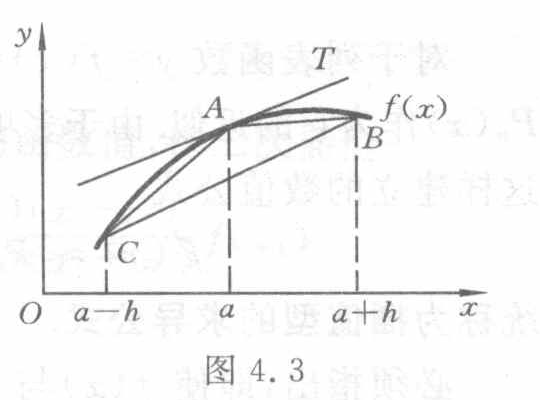
\includegraphics[width=0.85\linewidth,height=\textheight,keepaspectratio,alt={图 4.3（原书扫描裁切）}]{../assets/ch04b/figure-4-3.png}

图 4.3。原图标签：横轴 \(x\)、纵轴 \(y\)、原点 \(O\)；横轴位置 \(a-h\)、\(a\)、\(a+h\)，对应曲线上的点 \(C\)、\(A\)、\(B\)；曲线标记 \(f(x)\)，过 \(A\) 的切线标记 \(T\)。图中画出弦线 \(AB\)、\(AC\)、\(BC\) 与切线 \(AT\)。（此段为图中标签和图意的文字转录；原图未给出具体函数或数值。）

上述三种数值微分方法有个共同点，它们都是将导数的计算归结为计算 \(f\) 在若干节点上的函数值。这类数值微分方法称为机械求导方法。

要利用中点公式

\[
G(h)=\frac{f(a+h)-f(a-h)}{2h}
\]

计算导数 \(f'(a)\) 的近似值，首先必须选取合适的步长，为此需要进行误差分析。分别将 \(f(a\pm h)\) 在 \(x=a\) 处作 Taylor 展开，有

\[
f(a\pm h)=f(a)\pm hf'(a)+\frac{h^2}{2!}f''(a)
\pm\frac{h^3}{3!}f'''(a)+\frac{h^4}{4!}f^{(4)}(a)
\pm\frac{h^5}{5!}f^{(5)}(a)+\cdots,
\]

代入上式得

\[
G(h)=f'(a)+\frac{h^2}{3!}f'''(a)+\frac{h^4}{5!}f^{(5)}(a)+\cdots.
\]

\href{../../source-images/pdf-113.jpeg}{原页图像}

\subsubsection{4.5.1 中点方法（续）}\label{ux4e2dux70b9ux65b9ux6cd5ux7eed}

由此得知，从截断误差的角度看，步长越小，计算结果越准确。

再考察舍入误差，按中点公式计算。当 \(h\) 很小时，因 \(f(a+h)\) 与 \(f(a-h)\) 很接近，直接相减会造成有效数字的严重损失（参见 1.4 节）。因此，从舍入误差的角度来看，步长是不宜太小的。

例如，用中点公式求 \(f(x)=\sqrt{x}\) 在 \(x=2\) 处的一阶导数，有

\[
G(h)=\frac{\sqrt{2+h}-\sqrt{2-h}}{2h}.
\]

设取四位数字计算，结果如表 4.6（导数的准确值 \(f'(2)=0.353\,553\)）所示。

\textbf{表 4.6}

{\def\LTcaptype{none} % do not increment counter
\begin{longtable}[]{@{}rrrrrr@{}}
\toprule\noalign{}
\(h\) & \(G(h)\) & \(h\) & \(G(h)\) & \(h\) & \(G(h)\) \\
\midrule\noalign{}
\endhead
\bottomrule\noalign{}
\endlastfoot
\(1\) & \(0.366\,0\) & \(0.05\) & \(0.353\,0\) & \(0.001\) & \(0.350\,0\) \\
\(0.5\) & \(0.356\,4\) & \(0.01\) & \(0.350\,0\) & \(0.000\,5\) & \(0.300\,0\) \\
\(0.1\) & \(0.353\,5\) & \(0.005\) & \(0.350\,0\) & \(0.000\,1\) & \(0.300\,0\) \\
\end{longtable}
}

在表 4.6 中，\(h=0.1\) 的逼近效果最好，如果进一步缩小步长，则逼近的效果会越来越差。

\subsubsection{4.5.2 插值型的求导公式}\label{ux63d2ux503cux578bux7684ux6c42ux5bfcux516cux5f0f}

对于列表函数 \(y=f(x)\)（见表 4.7），运用插值原理，可以建立插值多项式 \(y=P_n(x)\) 作为它的近似。由于多项式的求导比较容易，取 \(P_n'(x)\) 的值作为 \(f'(x)\) 的近似值，这样建立的数值公式

\[
f'(x)\approx P_n'(x)
\tag{4.5.1}
\]

统称为插值型的求导公式。

\textbf{表 4.7}

{\def\LTcaptype{none} % do not increment counter
\begin{longtable}[]{@{}cccccc@{}}
\toprule\noalign{}
\(x\) & \(x_0\) & \(x_1\) & \(x_2\) & \(\cdots\) & \(x_n\) \\
\midrule\noalign{}
\endhead
\bottomrule\noalign{}
\endlastfoot
\(y\) & \(y_0\) & \(y_1\) & \(y_2\) & \(\cdots\) & \(y_n\) \\
\end{longtable}
}

必须指出，即使 \(f(x)\) 与 \(P_n(x)\) 的值相差不多，导数的近似值 \(P_n'(x)\) 与导数的真值 \(f'(x)\) 仍然可能差别很大，因而在使用求导公式（4.5.1）时应特别注意误差的分析。

依据插值余项定理，求导公式（4.5.1）的余项为

\[
f'(x)-P_n'(x)=\frac{f^{(n+1)}(\xi)}{(n+1)!}\omega_{n+1}'(x)
+\frac{\omega_{n+1}(x)}{(n+1)!}\frac{\mathrm{d}}{\mathrm{d}x}f^{(n+1)}(\xi),
\]

其中

\[
\omega_{n+1}(x)=\prod_{k=0}^{n}(x-x_i).
\]

在此余项公式中，由于 \(\xi\) 是 \(x\) 的未知函数，无法对其第二项 \(\dfrac{\omega_{n+1}(x)}{(n+1)!}\dfrac{\mathrm{d}}{\mathrm{d}x}f^{(n+1)}(\xi)\) 作出进一步的说明，因此，对于随意给出的点 \(x\)，误差 \(f'(x)-P_n'(x)\) 是无法预估的。但是，如果限定求某个节点 \(x_k\) 上的导数值，那么上面的第二项因 \(\omega_{n+1}(x_k)=0\) 而变为

（本句续下页。）

\begin{quote}
校注（agent 补充，CH04B-E004）：原页``其中''后的节点多项式印为 \(\prod_{k=0}^{n}(x-x_i)\)，乘积指标 \(k\) 与因子下标 \(i\) 不一致，已按原扫描保留。结合本页表 4.7 和下文 \(\omega_{n+1}(x_k)=0\)，应将因子写作 \((x-x_k)\)，或统一将乘积指标改为 \(i\)；这是原书疑似下标排印错误，非 OCR 错误。\href{../assets/ch04b/review-p113-product.png}{局部原扫描}。
\end{quote}

\href{../../source-images/pdf-114.jpeg}{原页图像}

\subsubsection{4.5.2 插值型的求导公式（续）}\label{ux63d2ux503cux578bux7684ux6c42ux5bfcux516cux5f0fux7eed}

零，这时有余项公式

\[
f'(x_k)-P_n'(x_k)=\frac{f^{(n+1)}(\xi)}{(n+1)!}\omega_{n+1}'(x_k).
\tag{4.5.2}
\]

下面仅仅考察节点处的导数值。为简化讨论，假定所给的节点是等距的。

\paragraph{1. 两点公式}\label{ux4e24ux70b9ux516cux5f0f}

设已给出两个节点 \(x_0,x_1\) 上面的函数值 \(f(x_0),f(x_1)\)，作线性插值公式

\[
P_1(x)=\frac{x-x_1}{x_0-x_1}f(x_0)+\frac{x-x_0}{x_1-x_0}f(x_1).
\]

对上式两端求导，记 \(x_1-x_0=h\)，有

\[
P_1'(x)=\frac1h[-f(x_0)+f(x_1)],
\]

于是有下列求导公式：

\[
P_1'(x_0)=\frac1h[f(x_1)-f(x_0)],\quad
P_1'(x_1)=\frac1h[f(x_1)-f(x_0)].
\]

而利用余项公式（4.5.2）知，带余项的两点公式是

\[
f'(x_0)=\frac1h[f(x_1)-f(x_0)]-\frac h2f''(\xi),
\]

\[
f'(x_1)=\frac1h[f(x_1)-f(x_0)]+\frac h2f''(\xi).
\]

\paragraph{2. 三点公式}\label{ux4e09ux70b9ux516cux5f0f}

设已给出三个节点 \(x_0,x_1=x_0+h,x_2=x_0+2h\) 上的函数值，作二次插值

\[
\begin{aligned}
P_2(x)={}&\frac{(x-x_1)(x-x_2)}{(x_0-x_1)(x_0-x_2)}f(x_0)
+\frac{(x-x_0)(x-x_2)}{(x_1-x_0)(x_1-x_2)}f(x_1)\\
&+\frac{(x-x_0)(x-x_1)}{(x_2-x_0)(x_2-x_1)}f(x_2),
\end{aligned}
\]

令 \(x=x_0+th\)，上式可表示为

\[
P_2(x_0+th)=\frac12(t-1)(t-2)f(x_0)-t(t-2)f(x_1)
+\frac12t(t-1)f(x_2),
\]

两端对 \(t\) 求导，有

\[
P_2'(x_0+th)=\frac1{2h}[(2t-3)f(x_0)-(4t-4)f(x_1)+(2t-1)f(x_2)].
\tag{4.5.3}
\]

这里撇号表示对变量 \(x\) 求导数。上式分别取 \(t=0,1,2\)，得到以下三种三点公式：

\[
P_2'(x_0)=\frac1{2h}[-3f(x_0)+4f(x_1)-f(x_2)],
\]

\[
P_2'(x_1)=\frac1{2h}[-f(x_0)+f(x_2)],
\]

（第三个公式续下页。）

\href{../../source-images/pdf-115.jpeg}{原页图像}

\subsubsection{4.5.2 插值型的求导公式（续）}\label{ux63d2ux503cux578bux7684ux6c42ux5bfcux516cux5f0fux7eed-1}

\paragraph{2. 三点公式（续）}\label{ux4e09ux70b9ux516cux5f0fux7eed}

\[
P_2'(x_2)=\frac1{2h}[f(x_0)-4f(x_1)+3f(x_2)],
\]

而带余项的三点求导公式为

\[
f'(x_0)=\frac1{2h}[-3f(x_0)+4f(x_1)-f(x_2)]+\frac{h^2}3f'''(\xi),
\]

\[
f'(x_1)=\frac1{2h}[-f(x_0)+f(x_2)]-\frac{h^2}6f'''(\xi),
\tag{4.5.4}
\]

\[
f'(x_2)=\frac1{2h}[f(x_0)-4f(x_1)+3f(x_2)]+\frac{h^2}3f'''(\xi),
\]

其中式（4.5.4）是我们所熟悉的中点公式。在三点公式中，它由于少用了一个函数值 \(f(x_1)\) 而引人注目。

用插值多项式 \(P_n(x)\) 作为 \(f(x)\) 的近似函数，还可以建立高阶数值微分公式

\[
f^{(k)}(x)\approx P_n^{(k)}(x),\quad k=1,2,\cdots.
\]

例如，将式（4.5.3）再对 \(t\) 求导一次，有

\[
P_2''(x_0+th)=\frac1{h^2}[f(x_0)-2f(x_1)+f(x_2)],
\]

于是有

\[
P_2''(x_1)=\frac1{h^2}[f(x_1-h)-2f(x_1)+f(x_1+h)],
\]

而带余项的二阶三点公式为

\[
f''(x_1)=\frac1{h^2}[f(x_1-h)-2f(x_1)+f(x_1+h)]-\frac{h^2}{12}f^{(4)}(\xi).
\tag{4.5.5}
\]

\subsubsection{4.5.3 实用的五点公式}\label{ux5b9eux7528ux7684ux4e94ux70b9ux516cux5f0f}

设已给出五个节点 \(x_i=x_0+ih,\allowbreak \quad i=0,\allowbreak 1,\allowbreak 2,\allowbreak 3,\allowbreak 4\) 上的函数值，重复同样的手续，不难导出下列五点公式：

\[
m_0=\frac1{12h}[-25f(x_0)+48f(x_1)-36f(x_2)+16f(x_3)-3f(x_4)],
\]

\[
m_1=\frac1{12h}[-3f(x_0)-10f(x_1)+18f(x_2)-6f(x_3)+f(x_4)],
\]

\[
m_2=\frac1{12h}[f(x_0)-8f(x_1)+8f(x_3)-f(x_4)],
\]

\[
m_3=\frac1{12h}[-f(x_0)+6f(x_1)-18f(x_2)+10f(x_3)+3f(x_4)],
\]

\[
m_4=\frac1{12h}[3f(x_0)-16f(x_1)+36f(x_2)-48f(x_3)+25f(x_4)].
\]

其中 \(m_i\) 代表一阶导数 \(f'(x_i)\) 的近似值，读者不难导出这些求导公式的余项。

再记 \(M_i\) 表示二阶导数 \(f''(x_i)\) 的近似值，二阶五点公式如下：

（公式续下页。）

\href{../../source-images/pdf-116.jpeg}{原页图像}

\subsubsection{4.5.3 实用的五点公式（续）}\label{ux5b9eux7528ux7684ux4e94ux70b9ux516cux5f0fux7eed}

\[
M_0=\frac1{12h^2}[35f(x_0)-104f(x_1)+114f(x_2)-56f(x_3)+11f(x_4)],
\]

\[
M_1=\frac1{12h^2}[11f(x_0)-20f(x_1)+6f(x_2)+4f(x_3)-f(x_4)],
\]

\[
M_2=\frac1{12h^2}[-f(x_0)+16f(x_1)-30f(x_2)+16f(x_3)-f(x_4)],
\]

\[
M_3=\frac1{12h^2}[-f(x_0)+4f(x_1)+6f(x_2)-20f(x_3)+11f(x_4)],
\]

\[
M_4=\frac1{12h^2}[11f(x_0)-56f(x_1)+114f(x_2)-104f(x_3)+35f(x_4)].
\]

对于给定的一张数据表，用五点公式求节点上的导数值往往可以获得满意的结果。五个相邻节点的选择原则，一般是在所考察的节点的两侧各取两个邻近的节点，如果一侧的节点数不足两个（即一侧只有一个节点或没有节点），则用另一侧的节点补足。

\textbf{例 4.4}　利用 \(f(x)=\sqrt{x}\) 的一张数据表，按五点公式求节点上的导数值 \(m_i\) 与 \(M_i\)，并与导数的准确值比较，如表 4.8 所示。

\textbf{表 4.8}

{\def\LTcaptype{none} % do not increment counter
\begin{longtable}[]{@{}
  >{\raggedleft\arraybackslash}p{(\linewidth - 10\tabcolsep) * \real{0.1667}}
  >{\raggedleft\arraybackslash}p{(\linewidth - 10\tabcolsep) * \real{0.1667}}
  >{\raggedleft\arraybackslash}p{(\linewidth - 10\tabcolsep) * \real{0.1667}}
  >{\raggedleft\arraybackslash}p{(\linewidth - 10\tabcolsep) * \real{0.1667}}
  >{\raggedleft\arraybackslash}p{(\linewidth - 10\tabcolsep) * \real{0.1667}}
  >{\raggedleft\arraybackslash}p{(\linewidth - 10\tabcolsep) * \real{0.1667}}@{}}
\toprule\noalign{}
\begin{minipage}[b]{\linewidth}\raggedleft
\(x_i\)
\end{minipage} & \begin{minipage}[b]{\linewidth}\raggedleft
\(f(x_i)\)
\end{minipage} & \begin{minipage}[b]{\linewidth}\raggedleft
\(m_i\)
\end{minipage} & \begin{minipage}[b]{\linewidth}\raggedleft
\(f'(x_i)\)
\end{minipage} & \begin{minipage}[b]{\linewidth}\raggedleft
\(M_i/\times10^3\)
\end{minipage} & \begin{minipage}[b]{\linewidth}\raggedleft
\(f''(x_i)/\times10^3\)
\end{minipage} \\
\midrule\noalign{}
\endhead
\bottomrule\noalign{}
\endlastfoot
\(100\) & \(10.000\,000\) & \(0.050\,000\) & \(0.050\,000\) & \(-0.247\,58\) & \(-0.250\,00\) \\
\(101\) & \(10.049\,875\) & \(0.049\,751\) & \(0.049\,752\) & \(-0.245\,91\) & \(-0.246\,30\) \\
\(102\) & \(10.099\,504\) & \(0.049\,507\) & \(0.049\,507\) & \(-0.241\,91\) & \(-0.242\,68\) \\
\(103\) & \(10.148\,891\) & \(0.049\,267\) & \(0.049\,266\) & \(-0.239\,58\) & \(-0.239\,16\) \\
\(104\) & \(10.198\,039\) & \(0.049\,029\) & \(0.049\,029\) & \(-0.236\,91\) & \(-0.235\,72\) \\
\(105\) & \(10.246\,950\) & \(0.048\,795\) & \(0.048\,795\) & \(-0.236\,66\) & \(-0.232\,36\) \\
\end{longtable}
}

\subsubsection{4.5.4 样条求导}\label{ux6837ux6761ux6c42ux5bfc}

我们知道，样条函数 \(S(x)\) 作为 \(f(x)\) 的近似函数，不但彼此的函数值很接近，导数值也很接近。例如，对于三次样条 \(S_3(x)\)，有

\[
|f^{(a)}(x)-S_3^{(a)}(x)|=O(h^{4-a})\qquad(a=0,1,2,3),
\]

因此，用样条函数建立数值微分公式是很自然的，即

\[
f^{(a)}(x)\approx S_3^{(a)}(x)\qquad(a=0,1,2,3).
\tag{4.5.6}
\]

与前述插值型微分公式（4.5.1）不同，样条微分公式（4.5.6）可以用来计算插值范围内任何一点 \(x\)（不仅是节点 \(x_i\)）上的导数值。对于等距分划

\[
\pi:a=x_0<x_1<x_2<\cdots<x_n=b,\quad x_{k+1}-x_k=h,
\]

三次样条 \(S_3(x)\) 在节点上的导数值 \(S_3'(x_k)=m_k\) 满足下列连续性方程组

（方程组续下页。）

\begin{quote}
校注（agent 补充，原表记法说明）：表 4.8 后两列表头按原扫描保留为 \(M_i/\times10^3\) 与 \(f''(x_i)/\times10^3\)，未改写原表头。表内数值对应导数乘 \(10^3\) 后的数值，例如 \(f''(100)=-1/(4\cdot100^{3/2})=-0.00025\)，表中列为 \(-0.25000\)；此说明仅解释该页缩放记法。\href{../assets/ch04b/review-table-4-8.png}{表 4.8 原扫描局部}。
\end{quote}

\href{../../source-images/pdf-117.jpeg}{原页图像}

\subsubsection{4.5.4 样条求导（续）}\label{ux6837ux6761ux6c42ux5bfcux7eed}

\[
m_{k-1}+4m_k+m_{k+1}=3(y_{k+1}-y_{k-1})/h,\quad k=1,2,\cdots,n-1.
\tag{4.5.7}
\]

设已给出端点处的一阶导数值 \(m_0=y_0',m_n=y_n'\)，则求解方程组（4.5.7）得出的 \(m_k\) 即可作为导数 \(f'(x_k)\) 的近似值。

\subsection{小结}\label{ux5c0fux7ed3}

本章介绍积分和微分的数值计算方法。我们知道，积分和微分是两种分析运算，它们都是用极限来定义的。数值积分和数值微分则归结为函数值的四则运算，从而使计算过程可以在计算机上完成。

处理数值积分和数值微分的基本方法是逼近法：设法构造某个简单函数 \(P(x)\) 近似 \(f(x)\)，然后对 \(P(x)\) 求积（求导）得到 \(f(x)\) 的积分（导数）的近似值。本章基于插值原理推导了数值积分和数值微分的基本公式。

插值求积公式分 Newton-Cotes 公式与 Gauss 公式两类。前者取等距节点，算法简单而容易编制程序。Gauss 公式的精度高，但节点没有规律。运用带权的 Gauss 公式，能把复杂的积分化简，还可以直接计算奇异积分。构造 Gauss 公式会碰到选取求积节点（所谓 Gauss 点）的困难。

梯形法是众所周知的一种简单的求积方法。可以看到，将二分过程中的梯形值适当进行加权平均，会获得高精度的积分值。运用这种外推加速技术的 Romberg 算法，在电子计算机上有着广泛的应用。

限于篇幅，本章略去了数值积分的一些重要内容，如奇异积分、振荡函数的积分等，这些内容在文献 {[}7{]} 中有较为详尽的论述。关于高维积分的数值计算，有兴趣的读者可参看文献 {[}8{]}。

\subsection{习题}\label{ux4e60ux9898}

\textbf{1.} 确定下列求积公式中的待定参数，使其代数精度尽量高，并指明所构造出的求积公式所具有的代数精度：

（1）

\[
\int_{-h}^{h}f(x)\,\mathrm{d}x\approx A_{-1}f(-h)+A_0f(0)+A_1f(h);
\]

（2）

\[
\int_{-2h}^{2h}f(x)\,\mathrm{d}x\approx A_{-1}f(-h)+A_0f(0)+A_1f(h);
\]

（3）

\[
\int_{-1}^{1}f(x)\,\mathrm{d}x\approx[f(-1)+2f(x_1)+3f(x_2)]/3;
\]

（4）

\[
\int_0^h f(x)\,\mathrm{d}x\approx h[f(0)+f(h)]/1+ah^2[f'(0)-f'(h)].
\]

\textbf{2.} 分别用梯形公式和 Simpson 公式计算下列积分：

（1）

\[
\int_0^1\frac{x}{4+x^2}\,\mathrm{d}x,\quad n=8;
\]

（2）

\[
\int_0^1\frac{(1-e^{-x})^{\frac12}}{x}\,\mathrm{d}x,\quad n=10;
\]

（第 2 题其余小题续下页。）

\begin{quote}
校注（agent 补充，CH04B-E005）：第 1 题（4）首项的分母在原扫描中明确印为``1''，故保留 \(h[f(0)+f(h)]/1\)。该处疑为原书排印错误：仅作排印一致性检查，当 \(f\equiv1\) 时，积分为 \(h\)，而所印右端为 \(2h\)，并且导数项为零；疑应将分母印为``2''。此处不求解题中参数或代数精度。\href{../assets/ch04b/review-p117-exercises.png}{习题原扫描局部}。
\end{quote}

\href{../../source-images/pdf-118.jpeg}{原页图像}

\subsection{习题（续）}\label{ux4e60ux9898ux7eed}

\textbf{2.（续）}

（3）

\[
\int_1^9\sqrt{x}\,\mathrm{d}x,\quad n=4;
\]

（4）

\[
\int_0^{\pi/6}\sqrt{4-\sin^2\varphi}\,\mathrm{d}\varphi,\quad n=6.
\]

\textbf{3.} 直接验证 Cotes 公式（4.2.4）具有五次代数精度。

\textbf{4.} 用 Simpson 公式求积分 \(\displaystyle\int_0^1 e^{-x}\,\mathrm{d}x\) 并估计误差。

\textbf{5.} 推导下列三种矩形求积公式：

\[
\int_a^b f(x)\,\mathrm{d}x=(b-a)f(a)+\frac{f'(\eta)}2(b-a)^2,
\]

\[
\int_a^b f(x)\,\mathrm{d}x=(b-a)f(b)-\frac{f'(\eta)}2(b-a)^2,
\]

\[
\int_a^b f(x)\,\mathrm{d}x=(b-a)f\left(\frac{a+b}2\right)+\frac{f''(\eta)}{24}(b-a)^3.
\]

\textbf{6.} 证明梯形公式（4.2.9）和 Simpson 公式（4.2.11）当 \(n\to\infty\) 时收敛到积分 \(\displaystyle\int_a^b f(x)\,\mathrm{d}x\)。

\textbf{7.} 用复化梯形公式求积分 \(\displaystyle\int_a^b f(x)\,\mathrm{d}x\)。要将积分区间 \([a,b]\) 分成多少等份，才能保证误差不超过 \(\varepsilon\)（不计舍入误差）？

\textbf{8.} 用 Romberg 方法计算积分 \(\displaystyle\frac2{\sqrt\pi}\int_0^1 e^{-x}\,\mathrm{d}x\)，要求误差不超过 \(10^{-5}\)。

\textbf{9.} 卫星轨道是一个椭圆，椭圆周长的计算公式是

\[
s=a\int_0^{\pi/2}\sqrt{1-\left(\frac ca\right)^2\sin^2\theta}\,\mathrm{d}\theta,
\]

其中 \(a\) 是椭圆的长半轴，\(c\) 是地球中心与轨道中心（椭圆中心）的距离。记 \(h\) 为近地点距离，\(H\) 为远地点距离，\(R=6\,371\ \mathrm{km}\) 为地球半径，则 \(a=(2R+H+h)/2,\quad c=(H-h)/2\)。

我国第一颗人造卫星近地点距离 \(h=439\ \mathrm{km}\)，远地点距离 \(2\,384\ \mathrm{km}\)，试求卫星轨道的周长。

\textbf{10.} 证明等式

\[
n\sin\frac\pi n=\pi-\frac{\pi^3}{3!\,n^2}+\frac{\pi^5}{5!\,n^4}-\cdots,
\]

试依据 \(n\sin\dfrac\pi n\)（\(n=3,6,12\)）的值，用外推算法求 \(\pi\) 的近似值。

\textbf{11.} 用下列方法计算积分 \(\displaystyle\int_1^3\frac{\mathrm{d}y}{y}\)，并比较结果。

（1）Romberg 方法；

（2）三点及五点 Gauss 公式；

（3）将积分区间分为四等份，用复化两点 Gauss 公式。

\textbf{12.} 用三点公式和五点公式求 \(f(x)=\dfrac1{(1+x)^2}\) 在 \(x=1.0,1.1\) 和 \(1.2\) 处的导数值，并估计误差。\(f(x)\) 的值由表 4.9 给出。

\textbf{表 4.9}

{\def\LTcaptype{none} % do not increment counter
\begin{longtable}[]{@{}
  >{\centering\arraybackslash}p{(\linewidth - 10\tabcolsep) * \real{0.1667}}
  >{\centering\arraybackslash}p{(\linewidth - 10\tabcolsep) * \real{0.1667}}
  >{\centering\arraybackslash}p{(\linewidth - 10\tabcolsep) * \real{0.1667}}
  >{\centering\arraybackslash}p{(\linewidth - 10\tabcolsep) * \real{0.1667}}
  >{\centering\arraybackslash}p{(\linewidth - 10\tabcolsep) * \real{0.1667}}
  >{\centering\arraybackslash}p{(\linewidth - 10\tabcolsep) * \real{0.1667}}@{}}
\toprule\noalign{}
\begin{minipage}[b]{\linewidth}\centering
\(x\)
\end{minipage} & \begin{minipage}[b]{\linewidth}\centering
\(1.0\)
\end{minipage} & \begin{minipage}[b]{\linewidth}\centering
\(1.1\)
\end{minipage} & \begin{minipage}[b]{\linewidth}\centering
\(1.2\)
\end{minipage} & \begin{minipage}[b]{\linewidth}\centering
\(1.3\)
\end{minipage} & \begin{minipage}[b]{\linewidth}\centering
\(1.4\)
\end{minipage} \\
\midrule\noalign{}
\endhead
\bottomrule\noalign{}
\endlastfoot
\(f(x)\) & \(0.250\,0\) & \(0.226\,8\) & \(0.206\,6\) & \(0.189\,0\) & \(0.173\,6\) \\
\end{longtable}
}

\begin{quote}
校注（agent 补充，CH04B-E006）：第 9 题的原扫描明确写 \(s=a\int_0^{\pi/2}\cdots\,\mathrm{d}\theta\)，本转录保留原式。若 \(s\) 表示文中的椭圆``周长''，该式疑漏系数 \(4\)：所印表达式对应四分之一周长；以 \(c=0\) 的圆作一致性检查，原式给出 \(\pi a/2\)，而圆周长为 \(2\pi a\)。仅记录原书公式疑误，不代做本题数值计算。\href{../assets/ch04b/review-p118-orbit.png}{局部原扫描}。
\end{quote}

\subsection{本节覆盖原页的校注记录}\label{ux672cux8282ux8986ux76d6ux539fux9875ux7684ux6821ux6ce8ux8bb0ux5f55}

下列记录按原页关联，含同页相邻小节的校注；计算时同时读取上文校注和完整原页。

\begin{itemize}
\tightlist
\item
  \texttt{CH04A-E01}：原书 PDF 页 97
\item
  \texttt{CH04A-E02}：原书 PDF 页 100
\item
  \texttt{CH04A-E03}：原书 PDF 页 102
\item
  \texttt{CH04A-E04}：原书 PDF 页 102
\item
  \texttt{CH04A-E05}：原书 PDF 页 104
\item
  \texttt{CH04A-E06}：原书 PDF 页 104
\item
  \texttt{CH04A-E07}：原书 PDF 页 102
\item
  \texttt{CH04B-E001}：原书 PDF 页 106
\item
  \texttt{CH04B-E002}：原书 PDF 页 108
\item
  \texttt{CH04B-E003}：原书 PDF 页 111
\item
  \texttt{CH04B-E004}：原书 PDF 页 113
\item
  \texttt{CH04B-E005}：原书 PDF 页 117
\item
  \texttt{CH04B-E006}：原书 PDF 页 118
\end{itemize}

\end{document}
